
\documentclass[12pt,a4paper]{amsart}

% \usepackage{everypage}
% \usepackage[firstpage]{draftwatermark}
% \SetWatermarkScale{4}
% \SetWatermarkLightness{.95}

\newcommand{\OU}{\mathcal L}
\usepackage{amsmath,amssymb}
\usepackage{bbm}
\usepackage{bibentry}
\usepackage{bm}
\usepackage{cleveref}
\usepackage{fullpage}
\usepackage{macros}
\usepackage{mathabx}
\usepackage{mathtools}
\usepackage{graphicx}

% \newcommand{\exppi}[2]{\euler^{i\scalarof{#1}{#2}}}
% \newcommand{\expmi}[2]{\euler^{-i\scalarof{#1}{#2}}}
% \newcommand{\Basis}{(\Omega,\mathcal F,\Prob,(\mathcal F(t)_{t \ge 0}))}
% \newcommand{\frametop}[1]{\small\frametitle{\insertframenumber. #1}}
% \newcommand{\aval}[1]{\absoluteval{#1}}
% \newcommand{\cadlag}{C\`ADL\`AG}
% \DeclarePairedDelimiter{\ceil}{\lceil}{\rceil}
% \DeclarePairedDelimiter{\floor}{\lfloor}{\rfloor}

%% \renewcommand{\indicator}[1]{\mathbbmss 1 _{#1}}
%% \newcommand{\pspace}{(\Omega,\mathcal F,\Prob)}
%% \newcommand{\timeint}{\mathcal I}
%% \newcommand{\traj}{\mathcal T}

% \newcommand{\calF}{\mathcal F}
% \newcommand{\bu}{\bm u}
% \renewcommand{\S}{\mathbb S}
% \newcommand{\Sfunctions}{\mathcal S}
% \newcommand{\Dspace}[2]{\mathbb D^{#1,#2}}
% \newcommand{\bx}{\bm x}
% \newcommand{\by}{\bm y}
% \newcommand{\bz}{\bm z}
% \newcommand{\Mof}[1]{\operatorname{Mat}\left(#1\times#1\right)}
% \newcommand{\MRof}[2]{\operatorname{Mat}\left(#1\times#2\right)}
% \newcommand{\sym}[1]{\operatorname{Sym}(#1)}
% \newcommand{\psym}[1]{\operatorname{Sym}_+(#1)}
% \newcommand{\ppsym}[1]{\operatorname{Sym}_{++}(#1)}
% \newcommand{\GLof}[1]{\operatorname{GL}(#1)}
\newcommand{\one}{\bm 1}

\theoremstyle{plain}% default
\newtheorem{thm}{Theorem}%[section]
\newtheorem{proposition}[thm]{Proposition}
\newtheorem{npar}{}%[section]
\theoremstyle{definition}
\newtheorem{definition}{Definition}%[section]
\theoremstyle{remark}
\newtheorem{remark}{Remark}
\newtheorem{example}{Example}


\title{Probability 2021 \\ Part 2 \\
Probability on the real interval,\\ convergence of distributions,\\ conditioning}
\author[G. Pistone]{Giovanni Pistone}
\address{de Castro Statistics, Collegio Carlo Alberto}
\email{giovanni.pistone@carloalberto.org}
\urladdr{https://www.giannidiorestino.it/}
\date{DRAFT \today}

\begin{document}
\maketitle
\tableofcontents

The problem of finding a rigorous mathematical model for infinite sequences of binary independent repeated trials (0-1 outcomes) was solved by Emile Borel in the first years of XX century, by using the Lebesgue integration theory, at that time new. That solution was further generalised by A. Kolmogorov in the thirties with the use of abstract measure theory but actually the Borel solution is fully usable: an important author such as Norbert Wiener still used it in  the fifties. Nowadays, it is quite common to think to all distribution as a result of a simulation, which consists precisely of transformation of the uniform distribution on the unit interval to some other distribution of interest.

Measure theory is presented in the lecture notes by Bertand
Lods. Other presentations are in W. Rudin
\cite[Ch. 11]{rudin:1987-3rd} and in P. Malliavin \cite[Ch.~I-II]{malliavin:1995}. See also the slides of these lectures.

\section{Bernoulli trials: the Borel construction}
\label{sec:borel}

Consider the infinite sample space $S^\N = \set{0,1}^\N$. Each sample point is an infinite sequence of 0 and 1, $x=(x_1,x_2,\dots)$. The coordinate projections are denoted by $X_t$, $t \in \N$ namely, $X_t(x) = x_t$. There is a natural projection $X^t \colon S^\N \to S^t = \set{0,1}^t$, $t \in \N$, given by $X^t(x_1,x_2,\dots) = (x_1,x_2,\dots,x_t)$.

\subsection{The Borel $\sigma$-algebra of $S$ }
\label{sec:borel-sigma-algebra}

If $\mathcal S_t$ is the set of all sub-sets of $S^t$, then $\mathcal G_t = (X^t)^{-1} \mathcal S_t$ is an algebra of sub-sets of $S^\N$. It holds $\mathcal G_s \subset \mathcal G_t$ if $s \leq t$. The union of all $\mathcal G_t$ is a field contained in the set of all sub-sets of $S^\N$, which is a $\sigma$-field. The intersection of all $\sigma$-fields of $S^\N$ that contain all $\mathcal G_t$ is a $\sigma$-field denoted $\mathcal G_\infty$, the Borel $\sigma$-field of $S^\N$. The Bernoulli measurable space is $(S^\N,\mathcal G_\infty)$.

\begin{example} This example shows why we look for a
  $\sigma$-algebra. For each given $x \in S^\N$, define the sequence
  of frequencies $f_n(x) = \frac 1 n \sum_{t=1}^n (x_t=1)$. The real
  sequence of frequencies $(f_n(x))_{n\in\N}$ either converges to a
  real number in $[0,1]$ or is oscillating. If it is oscillating,
  there exist rational numbers $a,b \in \Q$, $a < b$, such that the sequence is infinitely often above $1/a$ and infinitely often below $1/b$. The set $\setof{x \in S^\N}{f_m(x) \geq 1/a}$ belong to the field $\mathcal S_m$. The set where the inequality holds infinitely often is the set
\begin{equation*}
  \bigcap_{n\in\N} \bigcup_{m \geq n
    }\setof{x \in S^\N}{f_m(x) \geq 1/a} 
\end{equation*}
which belongs to $\mathcal G_\infty$. Same for the other bound. In conclusion, the set of non-convergence is
\begin{equation*}
  \bigcup_{a,b\in\Q,a<b}  \left(\left(\bigcap_{n\in\N} \bigcup_{m \geq n
    }\setof{x \in S^\N}{f_m(x) \geq 1/a}\right) \bigcap  \left(\bigcap_{n\in\N} \bigcup_{m \geq n
    }\setof{x \in S^\N}{f_m(x) \leq 1/b} \right)\right)
\end{equation*}
which belongs to $\mathcal G_\infty$. The set of convergence is the complementary set. 
\end{example}

\bigskip

\begin{example}[The Law of Large Numbers (LLN)] Assume there exists a probability measure $\Prob$ on $(S^\N,\mathcal G_\infty)$. The sequence of random variables $(f_n)_{n \in\N}$ satisfies the LLN if there exists a random variable $f_\infty$ such that $\probof{\setof{x \in S^\N}{\lim_{n\to\infty} f_n(x) = f(x)}} = 1$. The problem is well posed if the set $\setof{x \in S^\N}{\lim_{n\to\infty} f_n(x) = f(x)}$ is measurable. 
\end{example}

\bigskip

\begin{example}[Bernoulli shift] The mapping $T \colon S^\N \to S^\N$ defined by $T(x_1,x_2,x_3,\dots) = (x_2,x_3,\dots)$ is measurable. In fact, $T^{-1}(y_1,y_2,\dots) = \set{(0,y_1,y_2,\dots),(1,y_1,y_2,\dots)}$ hence $T^-1(\mathcal G_t) \subset \mathcal G_{t+1}$. The set where the LLN holds is invariant for the Bernoulli shift.  
\end{example}

\bigskip

\subsection{Bernoulli measure on the Bernoulli measurable space}
\label{sec:bern-meas-bern}

Given any
\begin{equation*}
  x = (x_1,x_2,\dots)\in \set{0,1}^\infty = S^\N \ ,
\end{equation*}
the series $\omega(x) = \sum_{t=1}^\infty x_t (1/2)^t$ is absolutely convergent to the real number $\omega$ in the interval $[0,1]$ whose expression in base 2 is  $(\omega)_2 = 0.x_1x_2\dots$ The mapping $\omega \colon S^\N \to [0,1]$ is not injective for example, $1/2=\sum_{k=2}^\infty (1/2)^k$. In binary notation, $.100\cdots = .011\cdots$.
The partial sum $\sum_{t=1}^n x_t (1/2)^t = \frac{\sum_{t=1}^k x_t 2^k}{2^n}$ is the left approximation of $\omega(x)$ by a binary rational. It follows that the mapping is surjective because for each $\omega \in [0,1]$ we can always construct a sequence $x$ such that $\omega(x)$ gives the required value. The mapping $\omega$ is a random variable from $(S^\N,\mathcal G_\infty)$ to $([0,1],\mathcal B)$, where $\mathcal B$ is a $\sigma$-algebra containing all binary intervals. In particular, every probability measure on $(S^\N,\mathcal G_\infty)$ has an image in $([0,1],\mathcal B)$.  

\begin{example}
  Consider the effect of the Bernoulli shift $T$. As $(T(x))_t = x_{t+1}$,
\begin{equation*}
  \omega(T(x)) = \sum_{t=1}^\infty x_{t+1}\left(\frac12\right)^t = 2 \sum_{s \geq 2} x_s \left(\frac12\right)^s = 2 \left(\omega(x) - \frac{x_1}2\right) = 2\omega(x) - X_1(x) \ .
\end{equation*}
It follows that
\begin{equation*}
X_1(x) = 2\omega(x) - \omega(T(x)) \ . 
\end{equation*}
In a similar way, one can prove that
\begin{equation*}
  X_2(x) = 2\omega(T^2(x)) - \omega(T^2(x)) \ ,
\end{equation*}
and so on.
\end{example}

\bigskip
\begin{example}[Simulation]
Let us provide the a measurable mapping $Y \colon [0,1] \to S^\N$ such that $\omega(Y(\theta)) = \theta$, $\theta \in [0,1]$. Let $H \colon \R \to \R$ be defined by $H(\theta)=0$ if $\theta \in ]-\infty,1[$ and $H(\theta)=1$ if $\theta \in [1/2,+\infty[$. One can check that
\begin{equation*}
  X_t(\theta) = H\left(2^t\theta - \sum_{j=1}^{t-1} X_j(\theta)2^{t-j} \right) \quad , \ t \in \N \ ,
\end{equation*}
is such that $\omega(X(\theta)) = \sum_{t=1}^\infty X_t(\theta) (1/2)^t = \theta$, where $X(\theta)$ is the sequence $(X_1(\theta), X_2(\theta), \dots) \in S^\N$. The set $\set{X_1 = 1}$ is the set of all $\omega \in [0,1]$ such that $2\omega \geq 1$ that is, $[1/2,1]$. The set $\set{X_1 = 1, X_2=1}$ is the set where $2\omega \geq 1$ and $4\omega - 2 \geq 1$ that is, $[3/4,1]$. The set ${X_1=0,X_2=1}$ is the set where $2\omega < 1$ and $4\omega \geq 1$ that is $[1/4,1/2[$. The set $\set{X_2=1}$ is $[1/4,1/2[ \cup [3/4,1]$.  
\end{example}

\bigskip

\begin{example} If $([0,1],\mathcal F,m)$ is the unit interval endowed with the Lebesgue measure, then
  \begin{equation*}
    \mathbb X \colon [0,1] \ni \omega \mapsto (X_j(\omega) \colon j \in \N)
  \end{equation*}
is a \emph{measurable function}. In fact, for all $t \in \N$ and all $x_1,\dots,x_t = 0,1$, the counter-image of the set
\begin{equation*}
  \setof{x \in S^\N}{X_1(x)=x_1,\dots,X_t(x)=x_t}
\end{equation*}
is a union of intervals. Here, measurable means that for each $B \mathcal S_\infty$ the set $\mathbb X^{-1}(B)$ is measurable in $[0,1]$. As a consequence, $B \mapsto \Prob(B) = m(\mathbb X^{-1}(B))$ is a probability measure on the Bernoulli measurable space. This follows from the following representation of the Bernoulli trials $X_t$. Let us consider the function on $[0,1]$ defined by $T(\omega) = 2\omega$ on $[0,1/2[$, $2\omega-1$ on $[1/2,1[$, and 0 at 1. Multiplying by 2 the equality $\omega = \sum_{t=1}^\infty X_t(\omega) \frac1{2^t}$ we get
\begin{equation*}
  2\omega = \sum_{t=1}^\infty X_t(\omega) \frac1{2^{t-1}} = \sum_{s=0}^\infty X_{s+1}(\omega) \frac1{2^{s}} = X_1(\omega) + \sum_{s=1}^\infty X_{s+1}(\omega) \frac1{2^{s}} 
\end{equation*}
$(S^\N,\mathcal S_\infty,\Prob)$ is the Bernoulli probability space with probability of success $1/2$.
\end{example}

\bigskip

\emph{Give any coherent family of probability measures on the sequence $S_t = \set{0,1}^t$, there exists a probability measure on $[0,1]$ whose images are the given measures.}

\begin{example}[Bernoulli trials]
Given the Bernoulli probabilities on $S^t$, compute the first images in $[0,1]$ and their distribution functions. Provide an intuitive argument to show that the sequence of distribution functions is convergent to a distribution function.  
\end{example}

\bigskip

\begin{example}[Independence of Bernoulli trials]
Show that the random variables $X_1,\dots,X_n$ are independent i.e., given functions $\phi_1,\dots,\phi_n \colon S \to \R$, it holds
\begin{equation*}
  \expectat p {\phi_1(X_1) \cdots \phi_n(X_n)} = \expectat p {\phi_1(X_1)} \cdots \expectat p {\phi_n(X_n)} \ .
\end{equation*}
\end{example}

\bigskip
\subsection{Weak LLN for Bernoulli trials}

Let $X_t$ be a sequence of Bernoulli trials with parameter $p$. It follows that $\probof{X_t=1} = p$ and $\expectat p {X_t} = p$. Define the frequences $F_n = \frac1n \sum_{t=1}^n X_t$. Then $\expectat p {F_n} = p$ and $\expectat p {\left(F_n - p\right)^2} = \frac {p(1-p)}n$. We have
\begin{equation*}
  1 - \probat p {p - \epsilon \leq F_n \leq p + \epsilon} \leq \frac1{n\epsilon^2} p(1-p) \ '
\end{equation*}
hence the limit as $n \to \infty$ of the rhs is 0.

\subsection{Strong LLN for Bernoulli trials}

Let us compute a better estimate of the probability of deviation from the mean value. For each $\beta \in \R$ we have
\begin{equation*}
  \expectat p {\euler^{\beta(F_n - a)}} = \euler^{-\beta a} \expectat p {\prod_{t=1}^n \euler^{\beta X_t/n}} = \euler^{-\beta a} \prod_{t=1}^n \expectat p {\euler^{\beta X_t/n}} = \euler^{-\beta a} \left((1-p)+ \euler^{\beta/n}p\right)^n  \ .
\end{equation*}
The $\log$ applied on both sides gives
\begin{equation*}
  \log \expectat p {\euler^{\beta(F_n - a)}} = -n\left(a \beta/n - \logof{(1-p) + \euler^{\beta/n} p}\right)  \ .
\end{equation*}
If we define
\begin{equation*}
  \kappa(a) = \sup \setof{a x - \logof{(1-p) + \euler^{x} p}}{x \in D} \ ,
\end{equation*}
we have the inequality
\begin{equation*}
\expectat p {\euler^{\beta(F_n - p)}} \leq \euler^{-n\kappa(a)} 
\end{equation*}
for all $\beta/n \in D$. Notice that the RHS is summable: $\sum_n \euler^{-nh(p)} < + \infty$.

The mapping $x \mapsto h(x) = ax - \logof{(1-p) + \euler^{x} p}$ has $h(0) = 0$ and has derivative
\begin{equation*}
h'(x) =  a - \frac{p \euler^x}{(1-p) + \euler^{x} p} \ ,
\end{equation*}
in particular $h'(0) = a - p$. The second derivative is negative i.e., the function is concave.

Let us apply the computations to the probabilities of deviations $F_n$ from $p$. One case is deviation at left. Write $a = p - \epsilon$ and $\beta/n \in ]-\infty,0[ = D$ to get
\begin{multline*}
  \probat p {F_n < p - \epsilon} = \probat p {F_n - a < 0} =   \\ \probat p {\beta(F_n-a) > 0} = \probat p {\euler^{\beta(F_n-a)} > 1} \leq \expectat p {\euler^{\beta(F_n-a)}} \leq \euler^{-n \kappa(a)} \ .
\end{multline*}

\begin{example}
  Conclude the argument above to prove the Strong LLN for Bernoulli trials.
\end{example}

\section{Distribution function and quantile function}
\label{sec:distr-funct-quant}

On the real measurable space $(\R,\mathcal B)$ we define the \emph{distribution function of the probability measure $\mu$} to be the real function $\R \ni x \mapsto F_\mu(x) = \mu(]-\infty,x])$. The distribution function of the real random variable $X$ is the distribution function of the induced probability measure, $F_X(x) = \probof{X \leq x}$. The class of intervals $\setof{]-\infty,x]}{x \in \R}$ is closed under intersection and generates the Borel $\sigma$-algebra $\mathcal B$. In fact $]-\infty, x] \cap ]-\infty,y] = ]-\infty,x \wedge y]$ and $]a,b[ = \cup_{n=1}^\infty ]-\infty,b-1/n] \setminus ] -\infty,a]$, hence $\mu=\nu$ if $F_\mu = F_\nu$.

\emph{The distribution function of $\mu$ has the following properties:
  \begin{enumerate}
  \item $\lim_{x \to -\infty} F_\mu(x) = 0$;
  \item $\lim_{x \to +\infty} F_\mu(x) = 1$;
  \item $(F_\mu(y) - F_\mu(x))(y-x) \geq 0$;
  \item $\lim_{y \downarrow x} F_\mu(y) = F_\mu(x)$;
  \item $\lim_{y \uparrow x} F_\mu(y) = \mu(]-\infty, x[)$.
\end{enumerate}}
Notice that $\mu\set{x} = F_\mu(x) - F_\mu(x-)$, that is, the discontinuity points are jumps and there is a concentrated [probability mass the point of discontinuity.

A generic function satisfying (1) to (5) is a \emph{distribution function}. We will show below that, conversely, \emph{any function $F \colon \R \to [0,1]$ with the properties 1) to 5) is a distribution function of a unique probability measure}. Distribution function on $\reals$ are, in a sense, similar to probability functions of a finite set in that they characterize the measure. But probability function are probability densities with respect ot a measure, while distribution function are not.

Given any distribution function $F$ and any real $t$ the set $\set{F \geq t} = \setof{x \in \R}{F(x) \geq t}$ is a left-closed interval $[Q(t),+\infty[$. In fact, $F(y) \geq t$ implies $F(z) \geq t$ for all $z \geq y$ and the minimum of $\setof{x \in \R}{F \geq t}$ obtains at some $Q(t) \in \R \cup \set{-\infty,+\infty}$. Notice that for all $x,t \in \reals$, $Q(t) \leq x$ is equivalent to $F(x) \geq t$ and $Q(t) < x$ is equivalent to $F(x) < t$. If $t \leq 0$, then $Q(t) = -\infty$; if $t > 1$ then $Q(t) = + \infty$; if $t \in ]0,1[$ then $Q(t)$ is finite; if $t=1$ then the relevant condition is $F(x) = 1$ hence $Q(1)$ can be either $+\infty$ of finite. The restriction of $Q$ to $]0,1[$ is called the \emph{quantile function of $F$}.

\emph{The quantile function is non-decreasing and left-continuous}. In fact: 1) $s < t$ implies $\setof{x\in\R}{F(x) \geq t} \subseteq \set{x\in\R}{F(x) \geq s}$ hence $Q(s) \leq Q(t)$; 2) $\setof{t \in ]0,1[}{Q(t) \leq x}$ is a (relatively) closed interval.

A non-decreasing function has at most a numerable many jump points. It can be seen by evaluating the number of jumps larger than a given $\epsilon > 0$. A non decreasing function is continuous in all points except a denuberable set.

As $Q(t) = \inf\setof{x \in \R}{F(x) \geq t}$, we have $Q(F(x)) = \inf\setof{y \in \R}{F(y) \geq F(x)} = x^- \leq x$. If $F$ is not invertible then $x^- < x$ for some $x$ and $F(Q(F(x))) = F(x)$. If $F$ is invertible, then $x^-=x$ and $Q = F^{-1}$.

\emph{Let $F$ be a distribution function with quantile function $Q$. Let $m$ be the Lebesgue probability measure on $]0,1[$ and let $\mu = Q_{\#} m$ be the image of $m$ under $q$. The distribution function of $\mu$ is $F$, $F_{Q_{\#} m} = F$.} In fact, $Q^{-1}(]-\infty,x]) = \setof{t \in ]0,1[}{Q(t) \leq x} = \setof{t \in ]0,1[}{F(x) \geq t} = ]0,F(x)]$ so that $m(Q^{-1}(]-\infty,x])) = F(x)$.

If $\mu$ is a probability measure on $(\R,\mathcal B)$ and $\phi$ is any integrable function then 
\begin{equation*}
  \int \phi(x) \ \mu(dx) = \int_0^1 \phi(Q(t)) \ dt \ .
\end{equation*}
If moreover $F_\mu \in C^1(\R)$ then the Change of Variable Theorem gives
\begin{equation*}
  \int \phi(x) \ \mu(dx) = \int_0^1 \phi(F_\mu^{-1}(t)) \ dt = \int_{F_\mu(-\infty)}^{F_\mu(+\infty)} \phi(x) F'_{\mu}(x) \ dx = \int_{F_\mu(-\infty)}^{F_\mu(+\infty)} \phi(x)f_{\mu}(x) \ dx \ ,
\end{equation*}
where $f_\mu = F'_\mu$ is the \emph{density} of $\mu$ with respect to the Lebesgue measure $m$. This is a special case of the general notion of density.

Notice that we have proved that \emph{every probability measure on $(\reals,\mathcal B)$ can be \emph{simulated} with the Lebesgue probability measure on $]0,1[$.}

\emph{Let $X$ be a non-negative random variable on $(\Omega,\mathcal A,\mathbb P)$ with distribution function $F_X$. Then,
\begin{equation*}
  \expectof X = \int_0^{+\infty} (1-F_X(t-)) \ dt
\end{equation*}}

Let $\mu_X$ be the distribution of $X$, that is $\mu_X = X_\# \mathbb P$. Then, by the change of variable equation,
\begin{equation*}
  \expectof X = \expectof {(X \geq 0 )X} = \int (x \geq 0) x \ \mu_X(dx)
\end{equation*}
Now use the Fubini theorem.
\begin{multline*}
  \int_0^\infty x \ \mu_X(dx) = \int_0^{+\infty} \left(\int (t \leq x) dt\right) \mu_X(dx) = \int_0^\infty dt \int (t \leq x)  \mu_X(dx) = \\ \int_0^\infty \mu_X([t,\infty[) \ dt = \int_0^\infty (1 - F_X(t-)) \ dt \ .  
\end{multline*}

\begin{example}
Let $X$ be a real random variable. For each positive $\theta > 0$, $\euler^{\theta X}$ is a positive random variable, with distribution function
\begin{equation*}
  \probof{\euler^{\theta X} \leq t} = \probof{X \leq \theta^{-1} \log t} = F_X(\theta^{-1} \log t) \ .
\end{equation*}
It follows that
\begin{align*}
  \expectof{\euler^{\theta X}} &= \int_0^\infty (1 - F_X(\theta^{-1} \log t-)) \ dt \\
 &= \int_0^\infty (1 - F_X^-(\theta^{-1} \log t)) \ dt \\
  &= \int_{-\infty}^{+\infty} (1 - F_X^-(s)) \ \theta s \euler^{\theta s} \ ds\ . 
\end{align*}
One can proceed further with the transformation $s = \theta^{-1} \log t$ in the RHS.
\end{example}

The previous example shows how to compute $\expectof {\phi\circ X}$ with the distribution function when $\phi$ is increasing. The following is another special case.

Assume $\phi$ continuously differentiable, $\phi \in C^1(\reals)$ and assume $\phi\circ X$ is integrable. Write
\begin{equation*}
    \phi(x) = \phi(0) + \int_0^x \phi'(u) \ du = \begin{cases}
      \phi(0) + \int (0 < u \leq x) \phi'(u) \ du & \text{if $x > 0$} \\ \phi(0) & \text{if $x=0$} \\
      \phi(0) - \int (x < u \leq 0) \phi'(u) \ du & \text{if ${x < 0}$}
    \end{cases}
\end{equation*}
With the kernel $K(u,x) = -(x < u \leq 0) + (0 < u \leq x)$, it holds
\begin{equation*}
\phi(x) = \phi(0) + \int K(u,x) \phi'(u) \ du \ .    
\end{equation*}

Fubini gives
\begin{align*}
    \int \phi(x) \ \mu(dx) &= \phi(0) + \int \left( \int K(u,x) \phi'(u) \ du\right) \ \mu(dx) \\
    &= \phi(0) + \int \phi'(u) \left(\int k(u,x) \ \mu(dx) \right) du \\  &= \phi(0) - \int_{-\infty}^0 \phi'(u) F(u-) \ du + \int_0^{\infty} \phi'(0) (1 - F(u-)) \ du 
\end{align*}

Notice that $F(u) = F(u-)$ almost everywhere because the number of jumps is denumerable. Hence, in the integral both give the same result.

\begin{example}
[Uniform distribution on an interval] Given $a < b$, $a,b \in \reals$, consider the distribution function
\begin{equation*}
U_{a,b}(x) = \begin{cases}
  0 & \text{if $x < a$} \\
  \dfrac{x-a}{b-a} & \text{if $a \leq x \leq b$} \\
  1 & \text{if $x > b$}
\end{cases}
\end{equation*}
This function is not differentiable, but it is a primitive,
\begin{equation*}
    U_{a,b}(x) = \int_{-\infty}^x \frac1{b-a} (a \leq u b) \ du
\end{equation*}
$U_{a,b}$ has \emph{finite variation}. The equation above shows that $U_{a,b}$ is the distribution function of the probability measure with density $u_{a,b}(u) = \frac1{b-a} (a \leq u \leq b)$ with respect to the Lebesgue measure.

The quantile function is
\begin{equation*}
    ]0,1[ \ni t \mapsto \frac {b - t}{b-a}
\end{equation*}
For each non-negative $\phi$,
\begin{equation*}
\int \phi(u) u_{a,b}(u) \ du = \int_0^1 \phi\left(\frac{b-t}{b-a}\right)  \ dt  
\end{equation*}
\end{example}

\section{Weak convergence}
\label{sec:weak-convergence}

Given a sequence of random variables $(X_n)$ and a real random variable $\phi$, we are frequently interested in the convergence of the expected values, that is, the convergence of the sequence $(\expectof{\phi \circ X_n})$. Denote by $\mu_n$ the distribution of $X_n$, by $F_n$ the distribution function of $\mu_n$, and by $Q_n$ the quantile function of $F_n$.

\begin{example} Consider three examples: $X_n \sim \delta_{1/n}$, $X_n \sim U_{-n,n}$, and $X_n \sim U_{-1/n,1/n}$. Compare the example with the theorem below.
\end{example}

\emph{Let $\mu$ and $\mu_n$, $n \in \N$ be real probability measures with distribution functions $F$ and $F_n$ and quantile functions $Q$ and $Q_n$, respectively. The following conditions are equivalent.
\begin{enumerate}
\item $\lim_{n\to\infty} Q_n = Q$ almost everywhere;
\item For all continuous and bounded $\phi$, $\phi \in C_{\text{b}}$, it holds $\lim_{n \to \infty} \int \phi \ d\mu_n = \int \phi \ d\mu$. This convergence is called \emph{weak convergence}, $\mu_n \to \mu$.
\item  $F_n$ converges to $F$ at all continuity points of $F$.
\end{enumerate}}

\begin{example}[Proof]
$(1) \Rightarrow (2)$: If $\phi \in C_{\text{b}}$,
\begin{equation*}
  \lim_{n \to \infty} \int \phi \ d\mu_n = \lim_{n\to\infty} \int_0^1 \phi(Q_n(t)) \ dt = \int_0^1 \phi(Q_n(t)) \ dt = \int \phi \ d\mu
\end{equation*}
by bounded convergence. $(2) \Rightarrow (3)$: Given $x \in \R$ and  $\epsilon > 0$ consider the functions $f,g \in C_{\text{b}}(\R)$ defined by
\begin{equation*}
  f(y) =
  \begin{cases}
  1 & \text{if $y \leq x-\epsilon$} \\
  - \frac1\epsilon(y - x) & \text{if $x - \epsilon < y < x$} \\
  0 & \text{if $y \geq x$} \\
  \end{cases}
 \qquad g(x) =
 \begin{cases}
  1 & \text{if $y \leq x$} \\
  - \frac1\epsilon (y - x - \epsilon) & \text{if $x < y < x + \epsilon$} \\
  0 & \text{if $y \geq x+\epsilon$} \\
  \end{cases}
\end{equation*}
As $f \leq \one_{]-\infty,x]} \leq g$,
\begin{equation*}
  \int f \ d\mu \leq F(x) \leq \int g \ d\mu  \quad \text{and} \quad   \int f \ d\mu_n \leq F_n(x) \leq \int g \ d\mu_n  
\end{equation*}
which in turn gives $\lim_{n \to \infty} \aval{F(x) - F_n(x)} = 0$ if $\lim_{\epsilon\to 0} \int (g-f) \ d\mu = 0$. $(3) \Rightarrow (1)$: Let $s$ be a continuity point of $Q$. For each $\epsilon > 0$ choose two continuity points of $F$, say $x,y$ such that $x < Q(s) < y$ and $y - x \leq \epsilon$. As $Q$ is continuous at $s$ there exists $t > s$ such that $Q(t) \leq y$. The first inequality is equivalent to $F(x) < s$ and the second one implies $s < F(y)$. It follows that $F_n(x) < s \leq F_n(y)$ that is $x < Q_n(s) \leq y$. It is important to remark that in the proof of $(2) \Rightarrow (3)$ we do not need the totality of function in $C_{\text b}$. We need only bounded continuous functions that separate points in the sense explained in the proof. 
\end{example}

\section{Conditioning}
\label{sec:conditioning}

In this section, we discuss the formalism of conditioning, see, for example,
\cite[Ch.~3]{ross:2010introduction10} and \cite[IV.2]{malliavin:1995}.

\begin{example}[Sub-$\sigma$-algebras in flipping two coins]
  \begin{table}
    \[
\begin{array}{|c|c|c|c|c|c|}
\hline
\mbox{Events} & \mbox{Trivial $\sigma$-algebra} & \mathcal A_1 & \mathcal A_2 & \mathcal A_3
& \mathcal P(\Omega) \\
\hline
\emptyset & \bullet & \bullet & \bullet & \bullet & \bullet \\
\{(0,0)\} & & & & \bullet & \bullet \\
\{(0,1)\} & & & & & \bullet \\
\{(1,0)\} & & & & & \bullet \\
\{(1,1)\} & & & & \bullet & \bullet \\
\{(0,0),(0,1)\} & & \bullet & & & \bullet \\
\{(0,0),(1,0)\} & & & \bullet & & \bullet \\
\{(0,0),(1,1)\} & & & & \bullet & \bullet \\
\{(0,1),(1,0)\} & & & & \bullet & \bullet \\
\{(0,1),(1,1)\} & & & \bullet & & \bullet \\
\{(1,0),(1,1)\} & & \bullet & & & \bullet \\
\{(0,0),(0,1),(1,0)\} & & & & \bullet & \bullet \\
\{(0,0),(0,1),(1,1)\} & & & & & \bullet \\
\{(0,0),(1,0),(1,1)\} & & & & & \bullet \\
\{(0,1),(1,0),(1,1)\} & & & & \bullet & \bullet \\
\Omega & \bullet & \bullet & \bullet & \bullet & \bullet \\
 \hline
\end{array}\]
\caption{Levels of information in flipping two coins: no information,
  first coin only, second coin only, number of ones (indistinguishable
  coins), full information.\label{tab:2coins}}
\end{table}
See \cref{tab:2coins} for an example of sub-$\sigma$-algebras in the
2-binary experiment.
\end{example}

\subsection{Conditional expectation}

The notion of conditioning appears in many instances but all cases can
be effectively seen to depend on the following, very general,
definition.

\begin{definition}[Conditional expectation wrt a $\sigma$-algebra]\label{def:condexp1}
  Let $(\Omega,\mathcal F,\mu)$ be a probability space. Given a
  sub-$\sigma$-algebra $\mathcal G$ and a real integrable random
  variable $X$, a \emph{version of the conditional expectation of $X$
    given $\mathcal G$} is an integrable real random variable
  $\widetilde X$ satisfying the following two conditions:
\begin{enumerate}
\item $\widetilde X$ is $\mathcal G$-measurable; and
\item for each bounded and $\mathcal G$-measurable real random variable
  $G$, it holds
  \begin{equation}\label{eq:conexp1}
    \expectof {XG} = \expectof{\widetilde X G} \ .
  \end{equation}
\end{enumerate}
\end{definition}

The previous definition provides a tool to actually compute
conditional expectation by writing down an integral equation. Notice
that it is enough to check \cref{eq:conexp1} on a convenient subset of
bounded $\mathcal G$-measurable real random variables $G$, for
example, all indicator function $G=\one_B$, $B \in \mathcal G$, or all
non-negative bounded $\mathcal G$-measurable real random variables.

\begin{example}[Trivial cases] The conditional expectation wrt the
  trivial $\sigma$-algebras is the ordinary expectation. The
  conditional expectation of the total $\sigma$-algebra is the identity.
  
\end{example}
\begin{example}[Symmetric $\sigma$-algebra]
  Let $(\reals,\mathcal B)$ be the real measurable space and consider a
  probability measure defined by a symmetric probability density,
  $\mu(A) = \int_A p(x) \ dx$ and $p(-x) = p(x)$. Let $\mathcal G$ be the
  $\sigma$-algebra of symmetric Borel sets, that is $\one_B(x) =
  \one_B(-x)$. The conditional expectation of the real random variable
  $f$ is defined by the integral equation
  \begin{equation*}
    \int f(x)\one_B(x) \ p(x)dx = \int \tilde f(x) \one_B(x) \ p(x)dx
    \ , \quad \text{$B$ symmetric.} 
  \end{equation*}
The solution is obtained by splitting the real line into two
half-lines and the reducing to the positive half-line:
\begin{equation*}
  \int_0^\infty (f(x)+f(-x)) \one_B(x) \ p(x)dx = 2 \int_0^\infty
  \tilde f(x) \one_B(x) \ p(x)dx \ .
\end{equation*}
Now $B \cap \reals_+$ is generic, so that $\tilde f(x) = \frac12 (f(x)
+ f(-x))$. Notice that the $\sigma$-algebra of symmetric Borel sets is
generated by the mapping $x \mapsto \aval x$.
\end{example}

\begin{example}[Exchangeable binary random variables] Consider the
  canonical binary process: $\Omega = \set{0,1}^n$,
  $\mathcal F = 2^\Omega$ (the family of all parts), $X_j(x) = x_j$,
$p$ a probability function on $\Omega$. Let $S_n$ be the group on
permutations of $\set{1,\dots,n}$. Let us say that a random variable
$G(X_1,\dots,X_n)$ is exchangeable if it is equal to
$G(X_{\sigma(1)},\dots,X_{\sigma(n)})$ for all $\sigma \in S_n$. One can check the following.  The set
of all exchangeable random variables is an algebra and the set of all
exchangeable sets is a $\sigma$-algebra, say $\mathcal S$. If the
probability function $p$ is exchangeable, then
$p(x_1,\dots,x_n) = \hat p(\sum_j x_j)$. In such a case, a version of
the conditional expectation of $F(X_1,\dots,X_n)$ is
\begin{equation*}
  \widetilde F(X_1,\dots,X_n) = \frac 1{n!} \sum_{\sigma \in S_n}
  F(X_{\sigma(1)},\dots,X_{\sigma(n)}) \ .  
\end{equation*}

\end{example}

\bigskip

Frequently, the sub-$\sigma$-algebra $\mathcal G$ is generated by a
random variable $Y$ with values in a measurable space $(E,\mathcal
E)$. In such a case, one uses the following result.

\begin{proposition}[Measurability lemma]
  Given measurable spaces $(\Omega,\mathcal F)$, $(E,\mathcal E)$,
  and a random variavle $Y \colon \Omega \to E$,
  $Y^{-1} \colon \mathcal E \to \mathcal F$, define
  $\mathcal G = \sigma(Y)$. A real function
  $\widetilde X \colon \Omega \to \reals$ is a $\mathcal G$-measurable
  real random variable if, and only if,
  $\widetilde X = \tilde f \circ Y$ for some measurable
  $\tilde f \colon E \to \reals$.
\end{proposition}

\begin{proof}
  If $\widetilde X = \tilde f \circ Y$, then
  ${\widetilde X}^{-1} = Y^{-1} \circ {\tilde f}^{-1}$, so that
  $\widetilde X$ is $\mathcal G$-measurable. Conversely, if
  $\widetilde X$ is $\mathcal G$-measurable, it is the poinwise limit
  of a sequence of simple $\mathcal G$-measurable real random variable
  each one of the form
  \begin{equation*}
    \sum_k a_k \one_{Y^{-1}(B_k)}= f \circ Y \ , \quad f = \sum_k a_k
    \one_{B_k} \ .
  \end{equation*}
  Finally, pointwise convergence holds true.
\end{proof}

In this case, the definition of conditional expectation is rephased as
follows.

\begin{definition}[Conditional expectation wrt a random variable]
Let $(\Omega,\mathcal F,\mu)$ be a probability space and $Y$ a random
variable with values in $(E,\mathcal E)$. Consider the
sub-$\sigma$-algebra $\sigma(Y) = Y^{-1} \mathcal E$. Given real integrable random variable $X$, a
\emph{version of the conditional expectation of $X$ given $Y$} is an integrable real random variable $\widetilde X$ satisfying the following two conditions:
\begin{enumerate}
\item $\widetilde X = \tilde f \circ Y$; and
\item for each bounded random variable of the form
  $g(Y)$, it holds
  \begin{equation*}
    \expectof {Xg(Y)} = \expectof{\tilde f(Y) g(Y)} \ .
  \end{equation*}
\end{enumerate}
\end{definition}

Notice that the lhs depends on the joint distribution of $X$ and $Y$,
while the RHS equals $\int \tilde f(y)g(y) \ \mu_Y(dy)$, where $\mu_Y$
is the distribution of $Y$, $\mu_Y= \mu \circ Y^{-1}$..

\begin{example}
Let $X$ be a real random variable whose distribution is uniform on
$[-1,1]$, that is, $\expectof {f(X)} = \frac12 \int_{-1}^1 f(x) \ dx$. Let us
compute a version of the conditional expectation of $X$ given $\aval
X$. Here $X = f(X)$ with $f(x) = x$. The distribution of $\aval X$ is uniform on $[0,1]$. The defining
equation is
\begin{equation*}
  \frac12 \int_{-1}^1 x g(\aval x) \ dx = \int_0^1 \tilde f(y) g(y) \
  dy  \ , 
\end{equation*}
so that $\widetilde f = 0$ because the integrand in the lhs is
anti-symmetric. 
\end{example}

\begin{example}
More generally, solve the same problem with $\expectof {f(X)} = \int_{-1}^1
f(x) \ p(x)dx$.
\end{example}

\begin{example}
Assume $(X_1,X_2)$ is Bernoulli$(\theta)$ and $S_2=X_1+X_2$. The
versions of the conditional expectation of $F(X_1,X_2)$ given $S_2$
are random variables of the form $\widetilde F(S_2)$ such that
\begin{equation*}
  \sum_{x_1,x_2 = 0,1} F(x_1,x_2) g(x_1+x_2) \theta^{x_1+x_2}
  (1-\theta)^{2 - (x_1 + x_2)} = \sum_{s=0}^2 \widetilde F(s) g(s)
  \binom 2 s \theta^s (1-\theta)^{2-s} \ ,
\end{equation*}
that is,
\begin{equation*}
 \sum_{s=0}^2 g(s) \theta^{s}
  (1-\theta)^{2 - s} \sum_{x_1,x_2 = 0,1, x_1+x_2 = s} F(x_1,x_2)  = \sum_{s=0}^2 \widetilde F(s) g(s)
  \binom 2 s \theta^s (1-\theta)^{2-s} \ .
\end{equation*}
A solution is $\widetilde F(s) = \binom 2 s ^{-1} \sum_{x_1,x_2 = 0,1,
  x_1+x_2 = s} F(x_1,x_2)$. Notice that the solution is unique in the case of full support, that is, $\theta \neq 0,1$.  
\end{example}

\subsection{Existence}
\label{sec:exists}

Let us prove the existence theorem for conditional expectation. This,
in turn, is a version of the Radon-Nikodym theorem in measure theory,
see \cite[Ch.~6]{rudin:1987-3rd}. Here is a recap of this topic.

Consider a measurable space $(\Omega,\mathcal F)$ and a finite measure
$\mu$ on it. If $p$ is a measurable, non-negative, $\mu$-integrable
random variable, then
\begin{equation*}
  \nu \colon \mathcal F \ni A \mapsto \int_A p \ d\mu = \int \one_Ap \
  \mu \ .
\end{equation*}
is a finite measure. In fact, $\sigma$-additivity depends on the
sequential continuity properties of the integral.

We can write $\nu = p \cdot \mu$ and say that $p$ is a version of the
density of $\nu$ with respect to $\mu$ or, a version of the derivative
of $\nu$ with respect to $\mu$. Two versions are $\mu$-a.e. equal. The
integrals wrt $p \cdot \mu$ are computed by
\begin{equation*}
  \int f \ d(p \cdot \mu) = \int f \ pd\mu \ .
\end{equation*}

The following existence theorem for the density holds true. See a proof in \cite{rudin:1987-3rd}

\begin{proposition}[Radon-Nikodym theorem]
If $\mu(A) = 0$, then $p \cdot \mu(A) = \int_A p \ d\mu =
0$. Conversely, if $\nu$ is a finite measure and $\mu(A) = 0$ implies
$\nu(A) =0$, then $\nu = p \cdot \nu$ for some density $p$. \end{proposition}

The relation $\nu = p \cdot \mu$ is also called absolute continuity
and written $\nu \ll \mu$.

Now, the existence of the conditional expectation is a simple
rephrasing of th existence of densities.

\begin{proposition}
With reference to \Cref{def:condexp1}, a version of the conditional expectation always exists.  
\end{proposition}

\begin{proof}
For each given integrable
$X$, write $X=X^+-X^-$ and $\mu_|$ for the restriction of $\mu$ to
$\mathcal G$. It is the probability measure on $(\Omega, \mathcal
G)$  defined by $\mu_|(B) = \mu(B)$.

Consider the finite measures
\begin{equation*}
  \chi_+(B) = \int_B X^+ \ d\mu \ , \quad \chi_-(B) = \int_B X^- \
  d\mu \ , \quad B \in
  \mathcal G \ .  
\end{equation*}
Both measures are absolutely continuous with respect to $\mu_|$. In
fact, if $\mu_|(B) = 0$, then $\mu(B)=0$ and, in turn, $\chi_+(B) = 0$
and $\chi_-(B)=0$. the quoted theorem implies that there exist $\mathcal G$-measurable densities $\widetilde{X^+}$
and $\widetilde{X^-}$ such that
\begin{equation*}
  \int_B \widetilde{X^+} \ d\mu = \int_B X^+ \ d\mu \quad \text{and} \quad
  \widetilde{X^-} = \int_B X^- \ d\mu \ , \quad  B \in \mathcal G \ .  
\end{equation*}
By taking the difference of the two equation and writing
$\widetilde{X}=\widetilde{X^+}-\widetilde{X^-}$ one get
\begin{equation*}
  \expectof{X G} = \expectof {\widetilde X G}
\end{equation*}
for all $G = \one_B$.
\end{proof}

%Let us prove the existence theorem.

% \begin{proposition}
% With reference to \Cref{def:condexp1}, a version of the conditional expectation always exists.  
% \end{proposition}

% \begin{proof}
% The exixtence follows immediatly from the Radon-Nikodym theorem, see,
% for example, \cite[Ch.~6]{rudin:1987-3rd}. For each given integrable
% $X$, write $X=X^+-X^-$ and $\mu_|$ for the restriction of $\mu$ to
% $\mathcal G$. It is the probability measure on $(\Omega, \mathcal
% G)$  defined by $\mu_|(B) = \mu(B)$.

% Consider the finite measures
% \begin{equation*}
%   \chi_+(B) = \int_B X^+ \ d\mu \ , \quad \chi_-(B) = \int_B X^- \
%   d\mu \ , \quad B \in
%   \mathcal G \ .  
% \end{equation*}
% Both measures are absolutely continuous with respect to $\mu_|$. In
% fact, if $\mu_|(B) = 0$, then $\mu(B)=0$ and, in turn, $\chi_+(B) = 0$
% and $\chi_-(B)=0$. the quoted theorem implies that there exist $\mathcal G$-measurable densities $\widetilde{X^+}$
% and $\widetilde{X^-}$ such that
% \begin{equation*}
%   \int_B \widetilde{X^+} \ d\mu = \int_B X^+ \ d\mu \quad \text{and} \quad
%   \widetilde{X^-} = \int_B X^- \ d\mu \ , \quad  B \in \mathcal G \ .  
% \end{equation*}
% By taking the difference of the two equation and writing
% $\widetilde{X}=\widetilde{X^+}-\widetilde{X^-}$ one get
% \begin{equation*}
%   \expectof{X G} = \expectof {\widetilde X G}
% \end{equation*}
% for all $G = \one_B$.
% \end{proof}

\begin{remark}
  Some Authors prefer to prove the existence of the conditional
  expectation with tools from Functional Analysis such as the
  existence of dual linear operators or the existence of
  projection. Given that, they derive the Radon-Nikodym theorem from
  a martingale convergence theorem, see, for example,
  \cite[\S~IV.2]{malliavin:1995}.
\end{remark}

Here are the first properties of conditional expectiation. Recall that
two random variables $X_1$ and $X_2$ of $(\Omega,\mathcal F,\mu)$ are
equal with probability 1 if $\probof{X_1 = X_2} = 1$. For real random
variables, the equality with probability 1 is equivalent to $\expectof{\aval{X_1-X_2}}=0$.

\begin{proposition}
  \begin{enumerate}\ 
  \item If $\probof{X_1 = X_2} = 1$ then $\probof{\widetilde X_1 =
      \widetilde X_2} = 1$.
%  \item  $\widetilde X_1$ and $\widetilde X_2$ are two versions of
%  the conditional expectation of the same $X$ if, and only if, $\probof{\widetilde X_1-\widetilde X_2=0}$.
  \item $\alpha \widetilde  X_1 + \beta \widetilde X_2$ is a version
    of the conditional expectation of $\alpha X_1 + \beta X_2$.
  \item If $\probof{X_1 \geq X_2} = 1$, then $\probof{\widetilde X_1 \geq
      \widetilde X_2} = 1$.
  \item If $\phi$ is convex, then $\probof{\phi\circ\widetilde X \leq
    \widetilde{\phi\circ X}} = 1$.
  \end{enumerate}
\end{proposition}

\begin{proof}
  \begin{enumerate}
  \item From $\expectof{X_1G} = \expectof{\widetilde X_1 G}$,
    $\expectof{X_2G} = \expectof{\widetilde X_2 G}$ and the
    assumption, we derive
    \begin{equation*}
      \expectof{(\widetilde X_1 - \widetilde X_2)G} =    \expectof{(
        X_1 - X_2)G} = 0 \ .
    \end{equation*}
Now, take $G = \Sgn(\widetilde X_1 - \widetilde X_2)$ to get $
\expectof{\aval{\widetilde X_1 - \widetilde X_2}} = 0$. 
%  \item From $\expectof{X_1G} = \expectof{\widetilde X_1 G}$,
%  $\expectof{X_2G} = \expectof{\widetilde X_2 G}$, we
%  derive \begin{equation*} 0 = \expectof{(\widetilde X_1 - \widetilde
%  X_2)G} 0 \ . \end{equation*} Now, take $G = \Sgn(\widetilde X_1 -
%  \widetilde X_2)$ to get $\expectof{\aval{\widetilde X_1 -
%  \widetilde X_2}} = 0$. Conversely, read the argument backwards.
  \item Linear combination preserves measurability and the expectation
    is linear, then the defining conditions check out.  
  \item Because of the previous property, it is enough to prove
    positivity. Assume $\probof{X \geq 0} = 1$ and $\probof{\widetilde
      X < 0} > 0$. It follows that
    \begin{equation*}
      0 \leq \expectof {X(\widetilde X < 0)} = \expectof{\widetilde X
        (\widetilde X < 0)} < 0 \ ,
    \end{equation*}
a contradiction.
  \item If $\phi$ is convex, there exist a function $\phi'$ (a
    sub-derivative) such that
    \begin{equation*}
      \phi(x) - \phi(y) \geq \phi'(y) (x-y) \ .
    \end{equation*}
It follows that
    \begin{equation*}
     \phi(X) - \phi(\widetilde X) \geq \phi'(\widetilde X)
      (X-\widetilde X) \ .
    \end{equation*}
    Now, moltiply by a non-negative $G$ and take the expectation.  It holds
  \begin{equation*}
    \expectof{(\phi(X) - \phi(\widetilde X))G} \geq \expectof{\phi'(\widetilde X)G
      (X-\widetilde X)} = 0 \ .
    \end{equation*}
Let us denote by $\widetilde{\phi\circ X}$ a version of the conditional
expectation of $\Phi\circ X$. Then,
\begin{equation*}
  0 \leq \expectof{(\phi\circ X - \phi \circ \widetilde X)G} =
  \expectof{(\widetilde{\phi\circ X} - \phi \circ \widetilde X)G} \ ,
\end{equation*}
which in turn, implies
\begin{equation*}
  \probof{\widetilde{\phi\circ X} \geq \phi \circ \widetilde X} = 1 \ .
\end{equation*}
  \end{enumerate}
\end{proof}

\begin{example}\label{ex:variogram}
Let $(X,Y)$ be uniformly distributed on the unit square $[0,1]^2$,
that is, $\expectof{F(X,Y)} = \iint_0^1 F(x,y) dx dy$.

We want to compute a version of the conditional expectation of
$F(X,Y)$ given the $\sigma$-algebra generated by $R = \aval{X-Y}$. The
defining equation is
\begin{equation*}
  \expectof{F(X,Y)g(\aval{X-Y})} = \expectof{\widetilde
  F(\aval{X-Y})g(\aval{X-Y})} \ ,
\end{equation*}
that is,
\begin{equation*}
  \iint_0^1 F(x,y)g(\aval{x-y}) \ dx dy  = \iint_0^1 \widetilde
  F(\aval{x-y})g(\aval{x-y}) \ dx dy \ .
\end{equation*}

Let us first consider the rhs. With the change of variable
\begin{equation*}
  \begin{cases}
    u  &= x - y \\ v &= y
  \end{cases}
  \qquad
  \begin{cases}
    x &= u + v \\ y &= v 
  \end{cases}
\end{equation*}
\begin{figure}
  \centering
  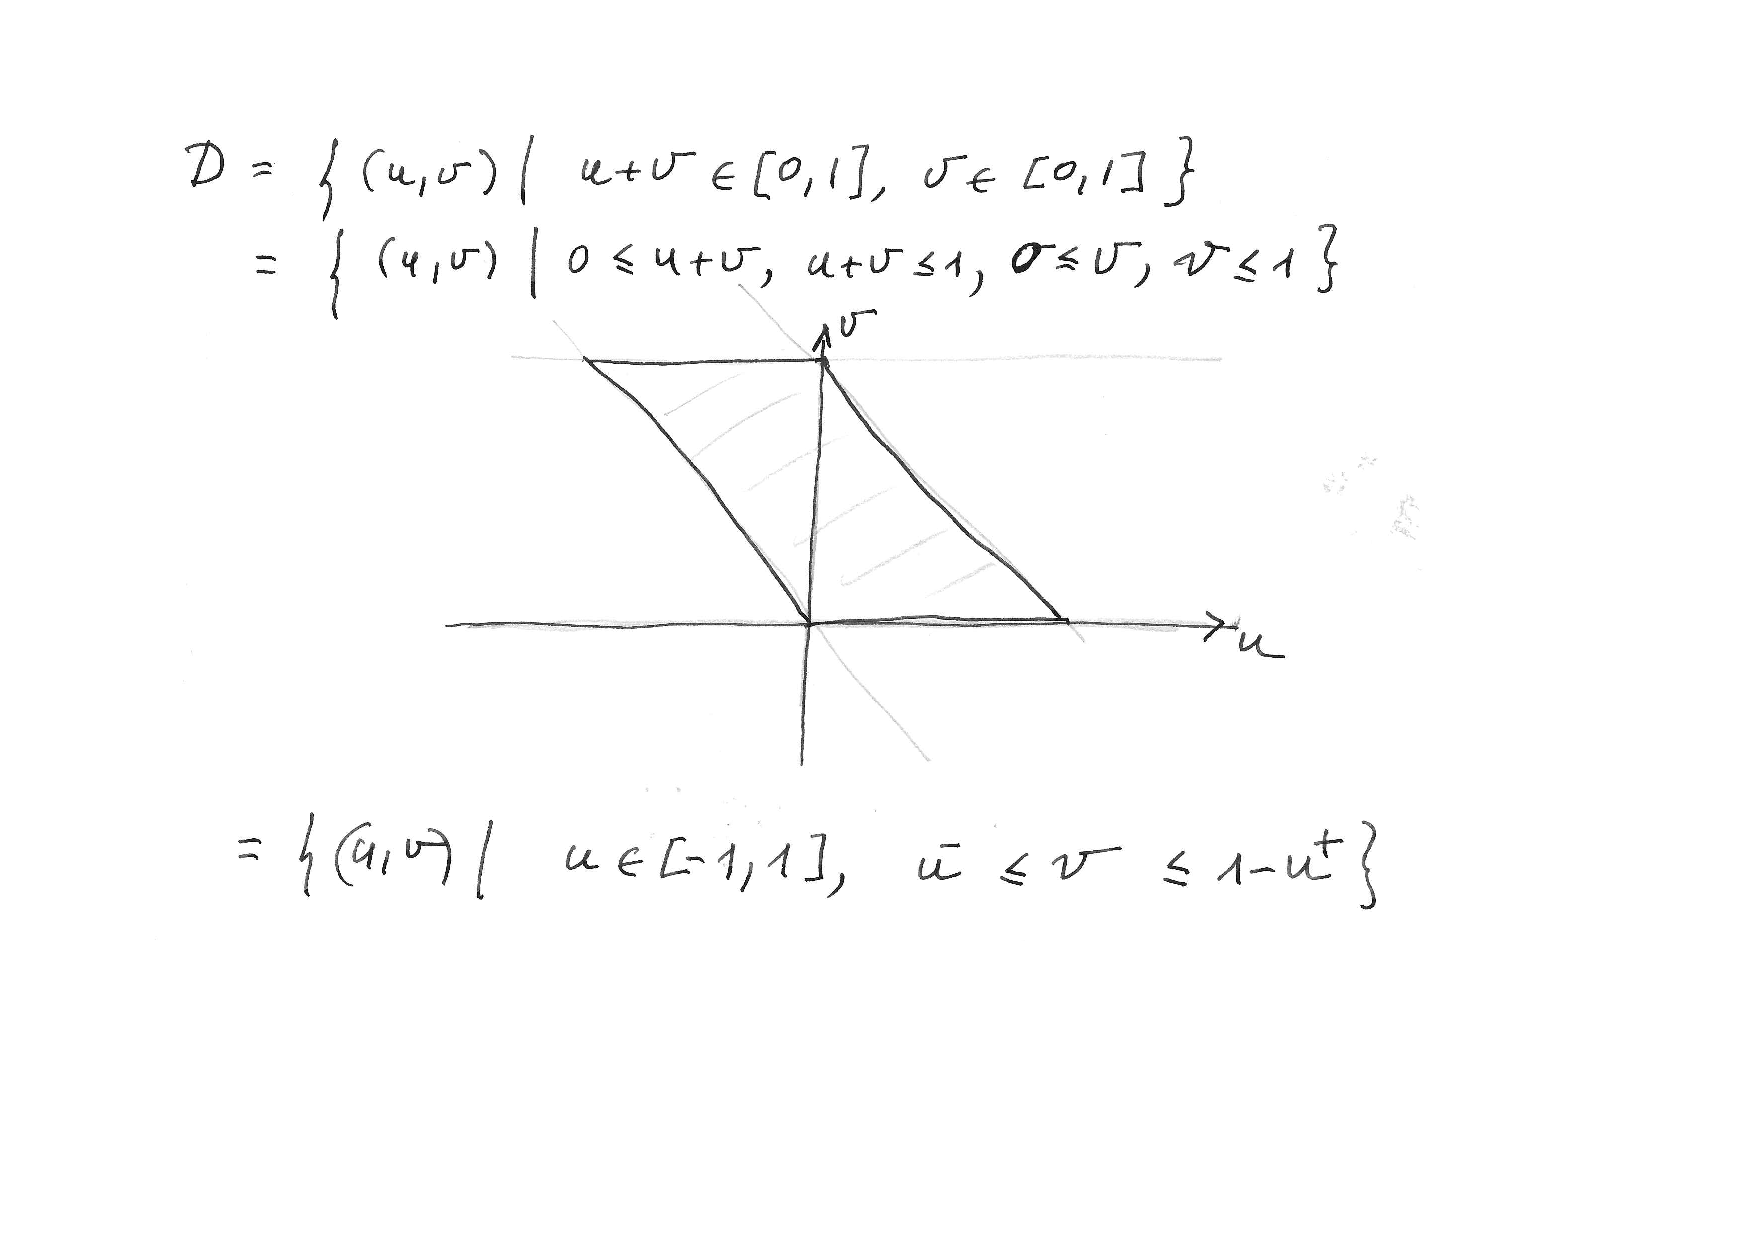
\includegraphics[height=.25\textheight]{pictures/domain.pdf}
  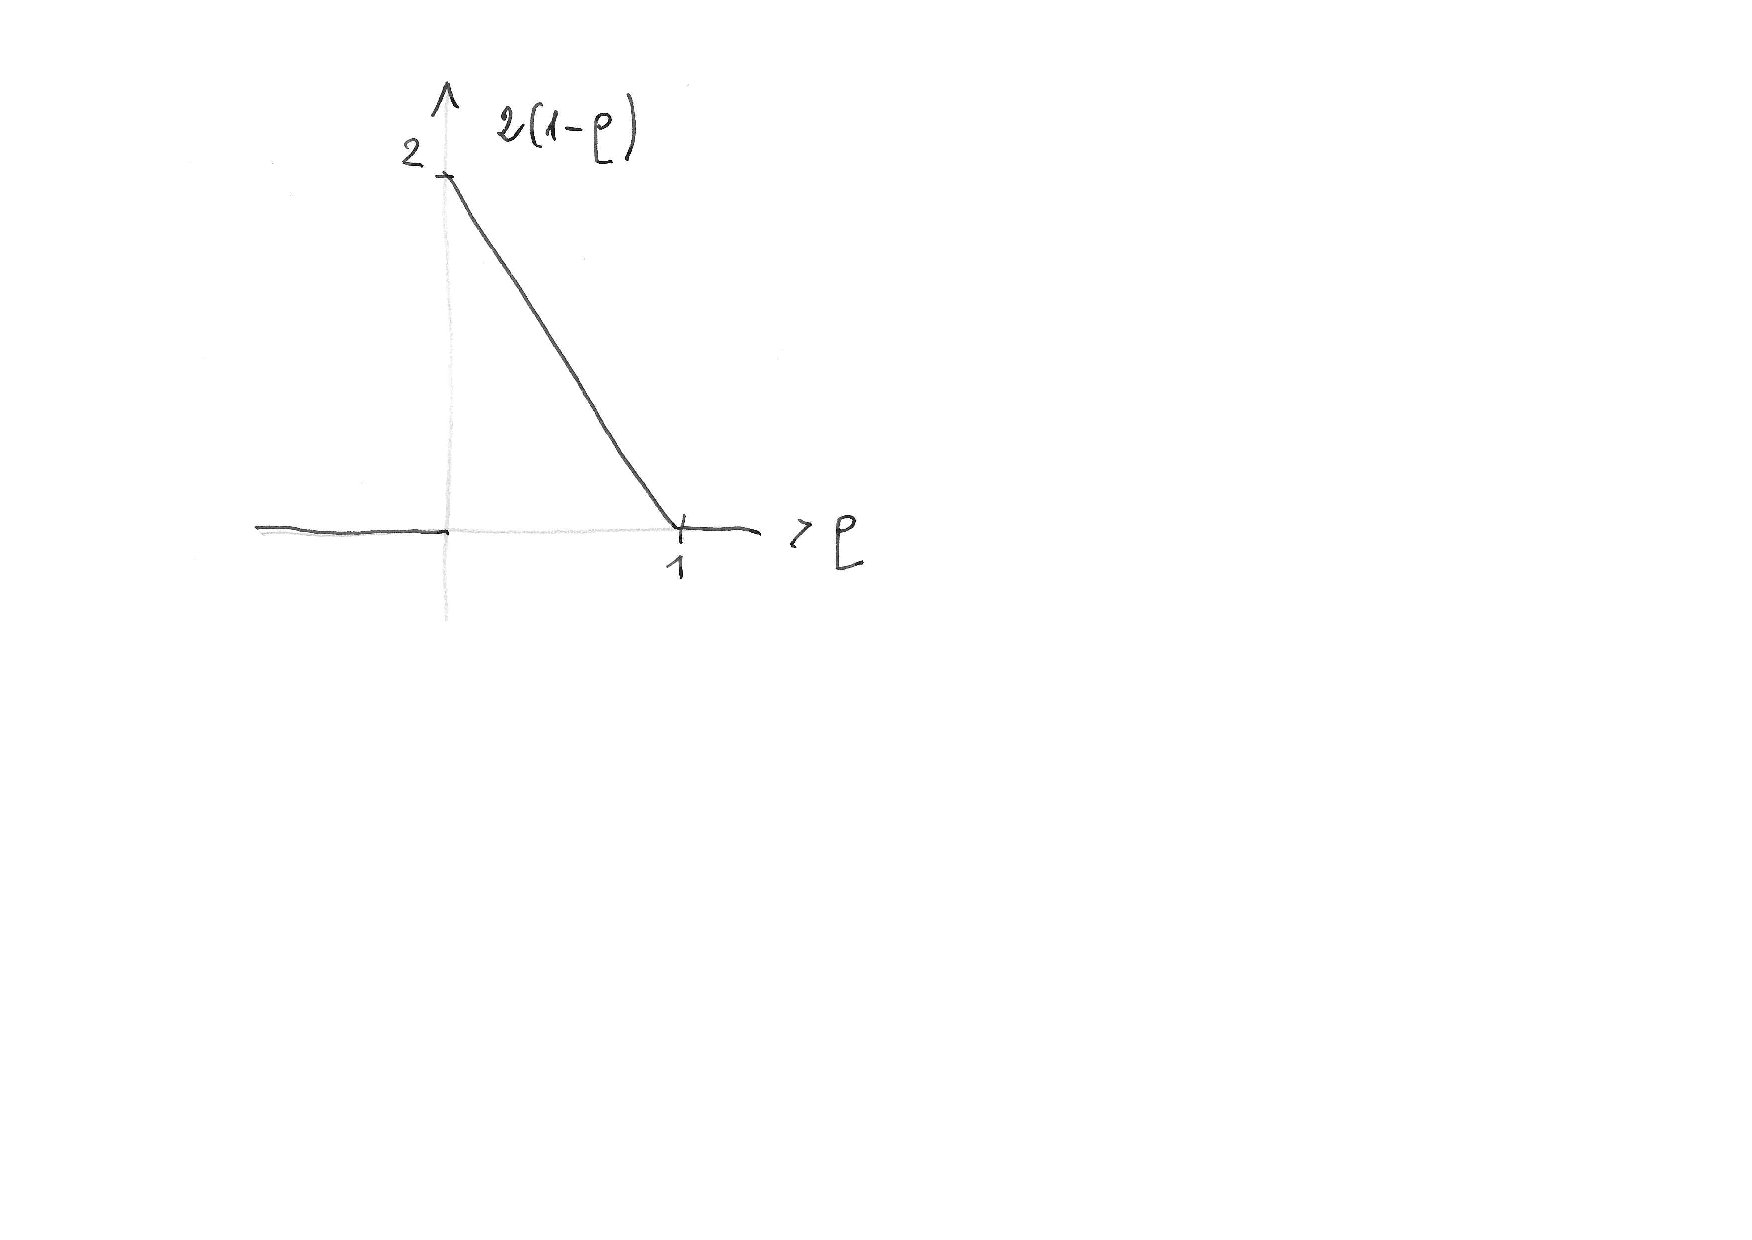
\includegraphics[height=.25\textheight]{pictures/density.pdf}
  \caption{Domain for \cref{ex:variogram}\label{fig:domain}}
\end{figure}
the image domain is (see \cref{fig:domain})
\begin{equation*}
  D = \setof{(u,v)}{-1 \leq u \leq 1, u^- \leq v \leq 1 - u^+} \ ,
\end{equation*}
and the integral becomes
\begin{multline*}
  \iint_0^1 \widetilde
  F(\aval{x-y})g(\aval{x-y}) \ dx dy = \int_D \widetilde F(\aval u)
  g(\aval u) \ du dv = \\ \int_{-1}^1 du \ \widetilde F(\aval u)
  g(\aval u) \int_{u^-}^{1-u^+} dv = \int_{-1}^1 \widetilde F(\aval u)
  g(\aval u) \ (1-\aval u) du \ .
\end{multline*}

The further change $\rho = \aval u$ is not invertible and we need to
split the integration domain in two parts, $-u = \rho$ if $u <0$ amd
$u = \rho$ otherwise, to get
\begin{multline*}
\int_{-1}^1 \widetilde F(\aval u)
  g(\aval u) \ (1-\aval u) du = \\ \int_{-1}^0 \widetilde F(- u)
  g(- u) \ (1+u) du + \int_0^1 \widetilde F(u)
  g(u) \ (1-u) du = \\  \int_0^1 \widetilde F(\rho)
  g(\rho) \ 2(1-\rho) d\rho \ .
\end{multline*}
In conclusion, the rhs is
\begin{equation*}
  \expectof{\widetilde
  F(\aval{X-Y})g(\aval{X-Y})} = \int_0^1 \widetilde F(\rho)
  g(\rho) \ 2(1-\rho) d\rho \ . 
\end{equation*}

The distribution of the conditioning variable $R = \aval{X-Y}$ is
$\mu_Y(d\rho) = 2(1-\rho) d\rho$. See a picture of the density in \cref{fig:domain}.

The same change of variable applied to the lhs produces
\begin{multline*}
  \iint_0^1 F(x,y)g(\aval{x-y}) \ dx dy = \\ \int_D F(u+v,v)
  g(\aval u) \ du dv = \int_{-1}^1 du \ g(\aval u)
  \int_{u^-}^{1-u^+} F(u+v,v) dv = \\ \int_{-1}^0 du \ g(-u)
  \int_{-u}^{1} F(u+v,v) dv + \int_0^1 du \ g(u)
  \int_0^{1-u} F(u+v,v) dv = \\
  \int_0^1 d\rho \ g(\rho)
  \int_{\rho}^{1} F(-\rho+v,v) dv + \int_0^1 du \ g(u)
  \int_0^{1-u} F(u+v,v) dv = \\
\int_0^1 d\rho \ g(\rho) \int_0^{1-\rho} dv \
\left(F(v,v+\rho)+F(v+\rho,v)\right) \ .\end{multline*}
\end{example}

In conclusion, equating the lhs and the rhs, we find
\begin{equation*}
  \widetilde F(\rho) = \frac1{2(1-\rho)} \int_0^{1-\rho} dv \
\left(F(v,v+\rho)+F(v+\rho,v)\right) \ . 
\end{equation*}

\subsection{The conditional expectation operator}

The relation between a class of $\mu$ equivalent random variables and
the corresponding class of equivalent versions of the conditional
expectations which has been established by the previous theorem,
allows to define the conditional expectation as an operator on
Lebesgue spaces.\footnote{We will skip some technical details related
  with the treatment of sets of outer probability 0}. `The result is
the following rephrasing of the proposition definition of conditional
expectation.

\begin{proposition}[Conditional expectation as an operator]\label{def:condexp3}
  Let $(\Omega,\mathcal F,\mu)$ be a probability space and let $\mathcal G$ be
  sub-$\sigma$-algebra $\mathcal G$. The \emph{conditional expectation
    operator} is the unique projection
  \begin{equation*}
    L^1(\mathcal F) \ni X \mapsto \condexp {X}{\mathcal G} \in
    L^1(\mathcal G)
  \end{equation*}
  such that
  \begin{equation*}
    \expectof{XG} = \expectof{\condexp{X}{\mathcal G}G} \ , \quad G
    \in L^\infty(\mathcal G) \ .
  \end{equation*}

  The conditional expectation operator has the following properties:
  \begin{enumerate}
  \item It is linear.
  \item It is positive.
  \item It satisfies Jensen inequality,
    \begin{equation*}
      \phi\left(\condexp{X}{\mathcal G}\right) \leq
      \condexp{\phi(X)}{\mathcal G} \ .
    \end{equation*}
\item If $\mathcal H$ is a sub-$sigma$-algebra of $\mathcal G$, that is,
  $\mathcal F \supset \mathcal G \supset \mathcal H$, then
  \begin{equation*}
    \condexp{\condexp X  {\mathcal G}}{\mathcal H} = \condexp X
    {\mathcal H} \ .
  \end{equation*}
  \end{enumerate}
\end{proposition}

\begin{proof}
Everything has been already proved but the last item. Let $\widetilde
X$ be a version of $\condexp X {\mathcal H}$ and let $\overline X$ be
a version of $\condexp X {\mathcal G}$. We want to prove that
$\widetilde X$ is a version of the conditional expectation of
$\overline X$ given $\mathcal H$. Now, $\widetilde X$ is indeed
$\mathcal H$-measurable. If $\widetilde {\overline X}$ is a version of
the conditional expectation of $\overline X$ given $\mathcal H$, then
for all $H$ bounded and $\mathcal H$-measurable, it holds
\begin{equation*}
  \expectof{\widetilde X  H} =  \expectof{X H} = \expectof {\overline
    X H} = \expectof{\widetilde{\overline X}H} \ ,
\end{equation*}
which implies $\probof{\widetilde X = \widetilde{\overline X}} = 1$.
\end{proof}

\begin{example}[Conditioning with respect to a partition] If the
  conditioning random variable is simple, say, taking values k values
  $y_1, \dot,y_k$, then the events $B_j={Y=y_j}$ form a partition of
  the sample space $\Omega$, and the $\sigma$-algebra generated by $Y$
  consists of all finite unions of elements of the partition. Every
  indicator function of a $B \in \sigma(Y)$ is of the form
  \begin{equation*}
    \one_B = \sum_{j=1}^k c_j \one_{B_j} \ , \quad c_j = 0,1 \ .
  \end{equation*}

The versions of the conditional expectation of a real random variable
$F(X)$ given $Y$ satisfy the master equation
\begin{equation*}
  \expectof{F(X)g(Y)} = \expectof{\widetilde F(Y)g(Y)} \ , 
\end{equation*}
that is, writing $g(Y) = \sum_j g(y_j)(Y=y_j)$ and $\widetilde F(Y) =
\sum_j F(y_j) (Y = y_j)$, 
\begin{equation*}
    \sum_{j=1}^k g(y_j) \expectof{F(X)(Y=y_j)} = \sum_{j=1}^k \widetilde
  F(y_j) g(y_j) \probof{Y=y_j} \ .
\end{equation*}
  It follows that $\widetilde F(y_j) \probof{Y= y_k} =
  \expectof{F(X)(Y=y-j)}$, that is, if all probabilities are positive,
  \begin{equation*}
    \widetilde F(Y) = \sum_{j=1}^k
    \frac{\expectof{F(X)(Y=y_j)}}{\probof{Y= y_k}}\one_{\set{Y=y_j}}\ . 
  \end{equation*}
This equation provides a definition of conditional expectation when
$X$ is generic and $Y$ simple. See a number of interesting examples in \cite[Ch.~3]{ross:2010introduction10}.
\end{example}

\begin{example} The argument in the existence proof above is actually of
  practical interest in the following case. Let $\mu$ and
  $\nu = p \cdot \mu$ both be probability measures on
  $(\Omega,\mathcal F)$. Consider a sub-$\sigma$-algebra
  $\mathcal G \subset \mathcal F$. As $\nu \ll \mu$, it holds
  $\nu_{|\mathcal G} \ll \mu_{|\mathcal G}$ and the density is a
  version of the conditional expectation $\widetilde p$. In fact, for
  all $B \mathcal G$ it holds
  \begin{equation*}
    \nu_{|\mathcal G}(B) = \nu(B) = \expectof{\one_B p} =
    \expectof{\one_B \tilde p} = \int_B \tilde p d\mu_{|\mathcal G} \ .
  \end{equation*}
\end{example}

\begin{example}[Equivalent measures] If $\nu \ll \mu$, with $\nu = p
    \cdot \mu$ and, moreover, $p > 0$, then $\mu \ll \nu$ with $\mu =
    \left(\frac1p\right) \cdot \nu$. In fact,
    \begin{equation*}
      \mu(A) = \int_A \frac p p \ d\mu = \int_A \frac1p \ d\nu \ .
    \end{equation*}
in this case, the two measures are equivalent, that is, $\mu(A) = 0$
if, and only if, $\nu(A) = 0$. This notion is interesting even in the
case of a finite state space and it is crucial in classical
statistics. A statistical model in a parameterized family of
probability models $\mu_\theta$, $\theta \in \Theta$ and the model is
almost always assumed to be ``regular'', that is, all the probability
measure are equivalent. In this case, one can chose a common reference
measure $\mu$ and write the model as $\mu_\theta = p_\theta \cdot
\mu$, with $p_\theta$ strictly positive, that is $p_\theta =
\euler^{u_\theta - \kappa(\theta)}$. This is the model studied in Part
1, but remember the difference between probability function and
probability model.  
\end{example}

\begin{example}[Changing probability]
  Consider the dependence of the conditional expectation from the
  given probability. Let $(\Omega,\mathcal F, \mu)$ be a probability
  space, $X$ and $Y$ two random variables, and assume
  $\widetilde f(Y)$ is a version of the conditional expectation of
  $f(X)$ given $Y$, that is,
  $\widetilde f(Y) = \condexpat \mu {f(X)}{Y}$. What about
  $\condexpat \nu {f(X)}{Y}$ for different probability measure $\nu$?

Assume absolute continuity $\nu \ll \mu$, that is $\nu = p \cdot
\mu$. Moreover, assume equivalence, $p > 0$, so that a $\mu$-version and
$\nu$-version is the same thing.

Let us write the master equation for $\nu$,
\begin{equation*}
  \expectat \nu {f(X) g(Y)} = \expectat \nu {\condexpat \nu {f(X)} Y
    g(Y)} \ .
\end{equation*}

The rhs is:
\begin{equation*}
\expectat \nu  {\condexpat \nu {f(X)} Y g(Y)} = \expectat \mu {p \condexpat
  \nu {f(X)} Y g(Y)} = \expectat \mu {\condexpat \mu p Y \condexpat \nu {f(X)}
  Y g(Y)}\ .
\end{equation*}

The lhs is
\begin{equation*}
  \expectat \nu {{f(X)} g(Y)} = \expectat \mu {p {f(X)} g(Y)} = \expectat \mu
  {\condexpat \mu {p{f(X)}} Y g(Y)} \ .
\end{equation*}

In conclusion,
\begin{equation*}
  \condexpat \mu p Y \condexpat {p \cdot\mu} {f(X)} Y = \condexpat \mu
  {p{f(X)}} Y \   
\end{equation*}
with $\mu$-probability 1. This is a generalization of Bayes formula. 

\end{example}


%\begin{example}[Changing probability with a density]
% Consider the dependence of the conditional expectation from the given
% probability. Let $(\Omega,\mathcal F, \mu)$ be a probability space,
% $X$ and $Y$ two random variables, and assume $\widetilde F(Y)$ is a
% version of the conditional expectation of $F(X)$ given $Y$, that is,
% $\widetilde F(Y) = \condexpat \mu {F(X)}{Y}$. What about $\condexpat \nu {F(X)}{Y}$ for different probability measure $\nu$?

% Assume absolute continuity $\nu << \mu$, that is $\nu = p \cdot \mu$.
% \end{example}

% \begin{example} The argument of the proof above is actually of
%   practical interest in the following case. Let $\mu$ and
%   $\nu = p \cdot \mu$ both be probability measures on
%   $(\Omega,\mathcal F)$. Consider a sub-$\sigma$-algebra
%   $\mathcal G \subset \mathcal F$. As $\nu \ll \mu$, it holds
%   $\nu_{|\mathcal G} \ll \mu_{|\mathcal G}$ and the density is a
%   version of the conditional expectation $\widetilde p$. In fact, for
%   all $B \mathcal G$ it holds
%   \begin{equation*}
%     \nu_{|\mathcal G}(B) = \nu(B) = \expectof{\one_B p} =
%     \expectof{\one_B \tilde p} = \int_B \tilde p d\mu_{|\mathcal G} \ .
%   \end{equation*}
% \end{example}

% \begin{example}[Equivalent measures] If $\nu \ll \mu$, with $\nu = p
%     \cdot \mu$ and, moreover, $p > 0$, then $\mu \ll \nu$ with $\mu =
%     \left(\frac1p\right) \cdot \nu$. In fact,
%     \begin{equation*}
%       \mu(A) = \int_A \frac p p \ d\mu = \int_A \frac1p \ d\nu \ .
%     \end{equation*}
% in this case, the two measures are equivalent, that is, $\mu(A) = 0$
% if, and only if, $\nu(A) = 0$. This notion is interesting even in the
% case of a finite state space and it is crucial in classical
% statistics. A statistical model in a parameterized family of
% probability models $\mu_\theta$, $\theta \in \Theta$ and the model is
% almost always assumed to be ``regular'', that is, all the probability
% measure are equivalent. In this case, one can chose a common reference
% measure $\mu$ and write the model as $\mu_\theta = p_\theta \cdot
% \mu$, with $p_\theta$ strictly positive, that is $p_\theta =
% \euler^{u_\theta - \kappa(\theta)}$. This is the model studied in Part
% 1, but remember the difference between probability function and
% probability model.  
% \end{example}

% \begin{example}[Changing probability]
%   Consider the dependence of the conditional expectation from the
%   given probability. Let $(\Omega,\mathcal F, \mu)$ be a probability
%   space, $X$ and $Y$ two random variables, and assume
%   $\widetilde f(Y)$ is a version of the conditional expectation of
%   $f(X)$ given $Y$, that is,
%   $\widetilde f(Y) = \condexpat \mu {f(X)}{Y}$. What about
%   $\condexpat \nu {f(X)}{Y}$ for different probability measure $\nu$?

% Assume absolute continuity $\nu \ll \mu$, that is $\nu = p \cdot
% \mu$. Moreover, assume equivalence, $p > 0$, so that a $\mu$-version and
% $\nu$-version is the same thing.

% Let us write the master equation for $\nu$,
% \begin{equation*}
%   \expectat \nu {f(X) g(Y)} = \expectat \nu {\condexpat \nu {f(X)} Y
%     g(Y)} \ .
% \end{equation*}

% The rhs is:
% \begin{equation*}
% \expectat \nu  {\condexpat \nu {f(X)} Y g(Y)} = \expectat \mu {p \condexpat
%   \nu {f(X)} Y g(Y)} = \expectat \mu {\condexpat \mu p Y \condexpat \nu {f(X)}
%   Y g(Y)}\ .
% \end{equation*}

% The lhs is
% \begin{equation*}
%   \expectat \nu {{f(X)} g(Y)} = \expectat \mu {p {f(X)} g(Y)} = \expectat \mu
%   {\condexpat \mu {p{f(X)}} Y g(Y)} \ .
% \end{equation*}

% In conclusion,
% \begin{equation*}
%   \condexpat \mu p Y \condexpat {p \cdot\mu} {f(X)} Y = \condexpat \mu
%   {p{f(X)}} Y \   
% \end{equation*}
% with $\mu$-probability 1. This is a generalization of Bayes formula. 

% \end{example}

 % measurable space such that for each positive or $\mu$-integrable
%  function $f \colon \Omega_2\times\Omega_2 \ni (x_1,x_2) \mapsto
%  f(x_1,x_2)$ it holds
%  \begin{equation*}
%      \int f \ d\mu = \int \left(\int f(x_1,x_2) \
%        \mu_{1|2}(dx_1|x_2)\right) \ \mu_2(dx_2) \ .
%    \end{equation*}
%    The measure $\mu$ is characterised on functions of the form
%    $f(x_1,x_2) = f_1(x_1)f_2(x_2)$ by
%    \begin{equation*}
%        \int f_1f_2 \ d\mu = \int \left(\int f_1(x_1) \
%          \mu_{1|2}(dx_1|x_2)\right)f_2(x_2) \ \mu_2(dx_2) \ .
%      \end{equation*}

%      measurable space such that for each positive or $\mu$-integrable
%  function $f \colon \Omega_2\times\Omega_2 \ni (x_1,x_2) \mapsto
%  f(x_1,x_2)$ it holds
%  \begin{equation*}
%      \int f \ d\mu = \int \left(\int f(x_1,x_2) \
%        \mu_{1|2}(dx_1|x_2)\right) \ \mu_2(dx_2) \ .
%    \end{equation*}
%    The measure $\mu$ is characterised on functions of the form
%    $f(x_1,x_2) = f_1(x_1)f_2(x_2)$ by
%    \begin{equation*}
%        \int f_1f_2 \ d\mu = \int \left(\int f_1(x_1) \
%          \mu_{1|2}(dx_1|x_2)\right)f_2(x_2) \ \mu_2(dx_2) \ .
%      \end{equation*}
%      [The proof is a simple variation of the argument for Fubini theorem.]

% A simple case occurs when the transition has the form
% \begin{equation*}
%     \mu_{1|2}(A_1|x_2) = \int_{A_1} p_{1|2}(x_1|x_2) \ \nu_1(dx),
%     \quad A_1 \in \mathcal F_1, x_2 \in \Omega_2 \,
%   \end{equation*}
%   where $(x_1,x_2) \mapsto p_{1|2}(x_1|x_2)$ is measurable on the
%   product space $(\Omega_1,\Omega_2, \mathcal F_1 \otimes \mathcal
%   F_2)$ and $x_1 \mapsto p_{1|2}(x_!|x_2)$ is a $\nu_1$-probability
%   density for each $x_2 \in \Omega_2$. In such a case,
%   \begin{multline*}
%     \int \left(\int f_1(x_1) \ \mu_{1|2}(dx_1|x_2)\right)f_2(x_2) \
%     \mu_2(dx_2) = \\ \int \left(\int f_1(x_1) p_{1|2}(x_1|x_2)
%       \nu_1(dx_1)\right)f_2(x_2) \ \mu_2(dx_2) = \\ \iint
%     f_1(x_1)f_2(x_2) p_{1|2}(x_1|x_2) \ \nu_1(dx_1) \mu_2(dx_2) \ ,
%   \end{multline*}
%   that is, $\mu = p_{1|2} \cdot \nu_1 \otimes \mu_2$. If moreover the
%   second measure has itself a density, $\mu_2 = p_2 \cdot \nu_2$, then
%   $\mu = (p_{1|2} \otimes p_2) \cdot \nu_1 \otimes \nu_2$
%   \begin{example}
%     % \begin{enumerate}
%     % \item
%       Let $T_1,T_2$ be independent and Exp$(1)$. Then the distribution
%       of $T_1$ given $T_1+T_1=t$ is uniform on $]0,t[$.
%       %  \item If $(Y_1,Y_2) \sim \normalof {n_1+n_2} 0 \Sigma$, $\det
%       %  \Sigma \ne 0$, find the conditional distribution of $Y_1$
%       %  given $Y_2$.
%       %  \item If $Y_1,Y_2$ are independent and $\normalof {} 0 1$,
%       %    find th \end{enumerate}
%     \end{example}

%     With the notations above, denoting with $X_1,X_2$ the coordinate
%     projection, the random variable $\widehat f(X_2) = \int f(x_1,X_2)
%     \ \mu_{1|2}(dx_1|X_2)$ is a version of the conditional expectation
%     $\condexpat \mu {f(X_1,X_2)}{\sigma(X_2)}$, namely a \emph{regular
%       version}. In fact,
%     \begin{equation*}
%           \expectat \mu {f(X_1,X_2)g(X_2)} = \int \left(\int
%             f(x_1,x_2) \ \mu_{1|2}(dx_1|x_2)\right)g(x_2) \
%           \mu_2(dx_2) = \expectat \mu {\widehat f(X_2)g(X_2)} \ .
%         \end{equation*}

\subsection{Transitions and conditional expectation}
\label{sec:trans-cond-expect}

 \begin{definition}
Given the product of two measurable spaces  \[(\Omega_1, \mathcal F_1)\otimes(\Omega_2, \mathcal F_2) = (\Omega_1\times\Omega_2, \mathcal F_1 \otimes \mathcal F_2)\] a \emph{transition} is a mapping $\mu_{1|2} \colon \mathcal F_1 \times \Omega_2 \to \reals$ such that
  \begin{enumerate}
  \item for each $x_2 \in \Omega_2$ the mapping $\mathcal F_1 \ni A_1 \mapsto \mu_{1|2}(A_1|x_2)$ is a probability measure on $(\Omega_1,\mathcal F_1)$ and
  \item for each $A_1 \in \mathcal F_1$ the mapping $\Omega_2 \ni x_2 \mapsto \mu_{1|2}(A_1|x_2)$ is $\mathcal F_2$-measurable.
  \end{enumerate}
\end{definition}

\begin{example}
In a sense, a transition is a generalization of the idea of point
function: insted of mapping $x_2 \mapsto f(x_2)$, one maps $x_2$ to a
probability measure $\mu_{1|2}(\cdot|x_2)$. Precisely, a deterministic
function $f$ corresponds to the transition $(A_1,x_2) \mapsto
\delta_{f(x_2)}(A_1) = (f(x_2) \in A_1)$. 
\end{example}

Each probability measure $\mu_{1|2}(\cdot|x_2)$ provides an
expectation \[x_2 \mapsto \condexp f {x_2} = \int f(x_1) \
  \mu_{1|w}(dx_1|x_2) \ .\]
It is easily seen that the resulting mapping is measurable. We will
see below that this is a form of conditional expectation.

Each probability measure in the transition can be specified in many
ways. For example:
\begin{enumerate}
\item If the space $(\Omega_1,\mathcal F_1)$ is finite, we can specify
  a transition probability function $(x_1,x_2) \mapsto p_{1|2}(x_1|x_2)$ such that 1) for each $x_2$
  the mapping $x_1 \mapsto p_{1|2}(x_1|x_2)$ is a probability function, and
  2) for each $x_1$ the mapping $x_2 \mapsto p_{1|2}(x_1|x_2)$ is
  measurable. In such a case, the transition will be defined
  by \[\mu_{1|2}(A|x_2) = \sum_{x_1 \in A} p_{1|2}(x_1|x_2) \quad \text{and}
    \quad \condexp {f} {x_2} = \sum_{x_1} f(x_1) p_{1|2}(x_1|x_2) \ .  \]
\item If the first space is a measure space $(\Omega_1,\mathcal F_1,
  \mu)$, we can specify a transition probability density $(x_1,x_2) \mapsto p_{1|2}(x_1|x_2)$ such that 1) for each $x_2$
  the mapping $x_1 \mapsto p_{1|2}(x_1|x_2)$ is a probability density, and
  2) for each $x_1$ the mapping $x_2 \mapsto p_{1|2}(x_1|x_2)$ is
  measurable. In such a case, the transition will be defined
  by \[\mu_{1|2}(A|x_2) = \int_A p_{1|2}(x_1|x_2) \ \mu(dx_1) \quad \text{and}
    \quad \condexp {f} {x_2} = \int f(x_1) p_{1|2}(x_1|x_2) \ \mu(dx_1)\ .  \]
\end{enumerate}

\begin{proposition}[Generalised Fubini]
Given a transition $\mu_{1|2}$ on $(\Omega_1\times\Omega_2, \mathcal F_1 \otimes \mathcal F_2)$ and a probability measure $\mu_2$ on $(\Omega_2,\mathcal F_2)$, there exists a unique probability measure $\mu = \int \mu_{1|2} \ d\mu_2$ on the product measurable space such that for each positive or $\mu$-integrable function $f \colon \Omega_2\times\Omega_2 \ni (x_1,x_2) \mapsto f(x_1,x_2)$ it holds
\begin{equation*}
  \int f \ d\mu = \int \left(\int f(x_1,x_2) \ \mu_{1|2}(dx_1|x_2)\right) \ \mu_2(dx_2) \ .
\end{equation*}
The measure $\mu$ is characterised on functions of the form $f(x_1,x_2) = f_1(x_1)f_2(x_2)$ by 
\begin{equation*}
  \int f_1f_2 \ d\mu = \int \left(\int f_1(x_1) \ \mu_{1|2}(dx_1|x_2)\right)f_2(x_2) \ \mu_2(dx_2) \ .
\end{equation*}
\end{proposition}

\begin{proof}
The proof is a simple variation of the argument for Fubini
theorem. Here are the main steps.
\begin{enumerate}
\item For each $A \in \mathcal F_1 \otimes \mathcal F_2$ and each $x_2
  \in \Omega_2$ the section $A_{x_2} = setof{x_1 \in
    \Omega_1}{(x_1,x_2) \in A}$ belongs to $\mathcal F_1$,
  \item The mapping $x_2 \mapsto \mu_{1|2}(A_{x_2}|x_2)$ is
    measurable.
  \item The mapping $A \mapsto \int \mu_{1|2}(A_{x_2}|x_2) \
    \mu(dx_2)$ is a probalility measure.
\end{enumerate}
Now the iterated integration formula and the characteriztion are
proved first by considering simple random variables and then taking limits.
\end{proof}

A simple case occurs when the transition has the form
\begin{equation*}
  \mu_{1|2}(A_1|x_2) = \int_{A_1} p_{1|2}(x_1|x_2) \ \nu_1(dx), \quad A_1 \in \mathcal F_1, x_2 \in \Omega_2 \,
\end{equation*}
where $(x_1,x_2) \mapsto p_{1|2}(x_1|x_2)$ is measurable on the product space $(\Omega_1,\Omega_2, \mathcal F_1 \otimes \mathcal F_2)$ and $x_1 \mapsto p_{1|2}(x_!|x_2)$ is a $\nu_1$-probability density for each $x_2 \in \Omega_2$. In such a case,  
\begin{multline*}
\int \left(\int f_1(x_1) \ \mu_{1|2}(dx_1|x_2)\right)f_2(x_2) \ \mu_2(dx_2) = \\ \int \left(\int f_1(x_1) p_{1|2}(x_1|x_2) \nu_1(dx_1)\right)f_2(x_2) \ \mu_2(dx_2) = \\ \iint f_1(x_1)f_2(x_2) p_{1|2}(x_1|x_2) \ \nu_1(dx_1) \mu_2(dx_2) \ ,
\end{multline*}
that is, $\mu = p_{1|2} \cdot \nu_1 \otimes \mu_2$.

If moreover the second measure has itself a density,
$\mu_2 = p_2 \cdot \nu_2$, then
$\mu = (p_{1|2} \otimes p_2) \cdot \nu_1 \otimes \nu_2$. This is the
elementary case $p_{12}(x_1,x_2) = p_{1|2}(x_1|x_2)p_2(x_2)$ which is
sometimes used to reverse the process,
$p_{1|2}(x_1|x_2) = p_{12}(x_1,x_2)/p_2(x_2)$.

\begin{example}[Bayes argument] The Bayes argument runs as
  follows. Given a \emph{model} $\mu_{1|2}$ and an \emph{apriori}
  $\mu_2$, one computes the joint $\mu_{12} = \mu_{1|2} \otimes \mu_2$ via Fubini. Then looks
  for the reverse representation by computing first the margin $\mu_1$
  of $\mu_{12}$ and looks for a representation of the form $\mu_{12} =
  \mu_{2|1} \otimes \mu_1$.  
 \end{example}

 \begin{example}[Exponential times and counting process]
   \label{ex:exponential}
\begin{figure}
  \centering
  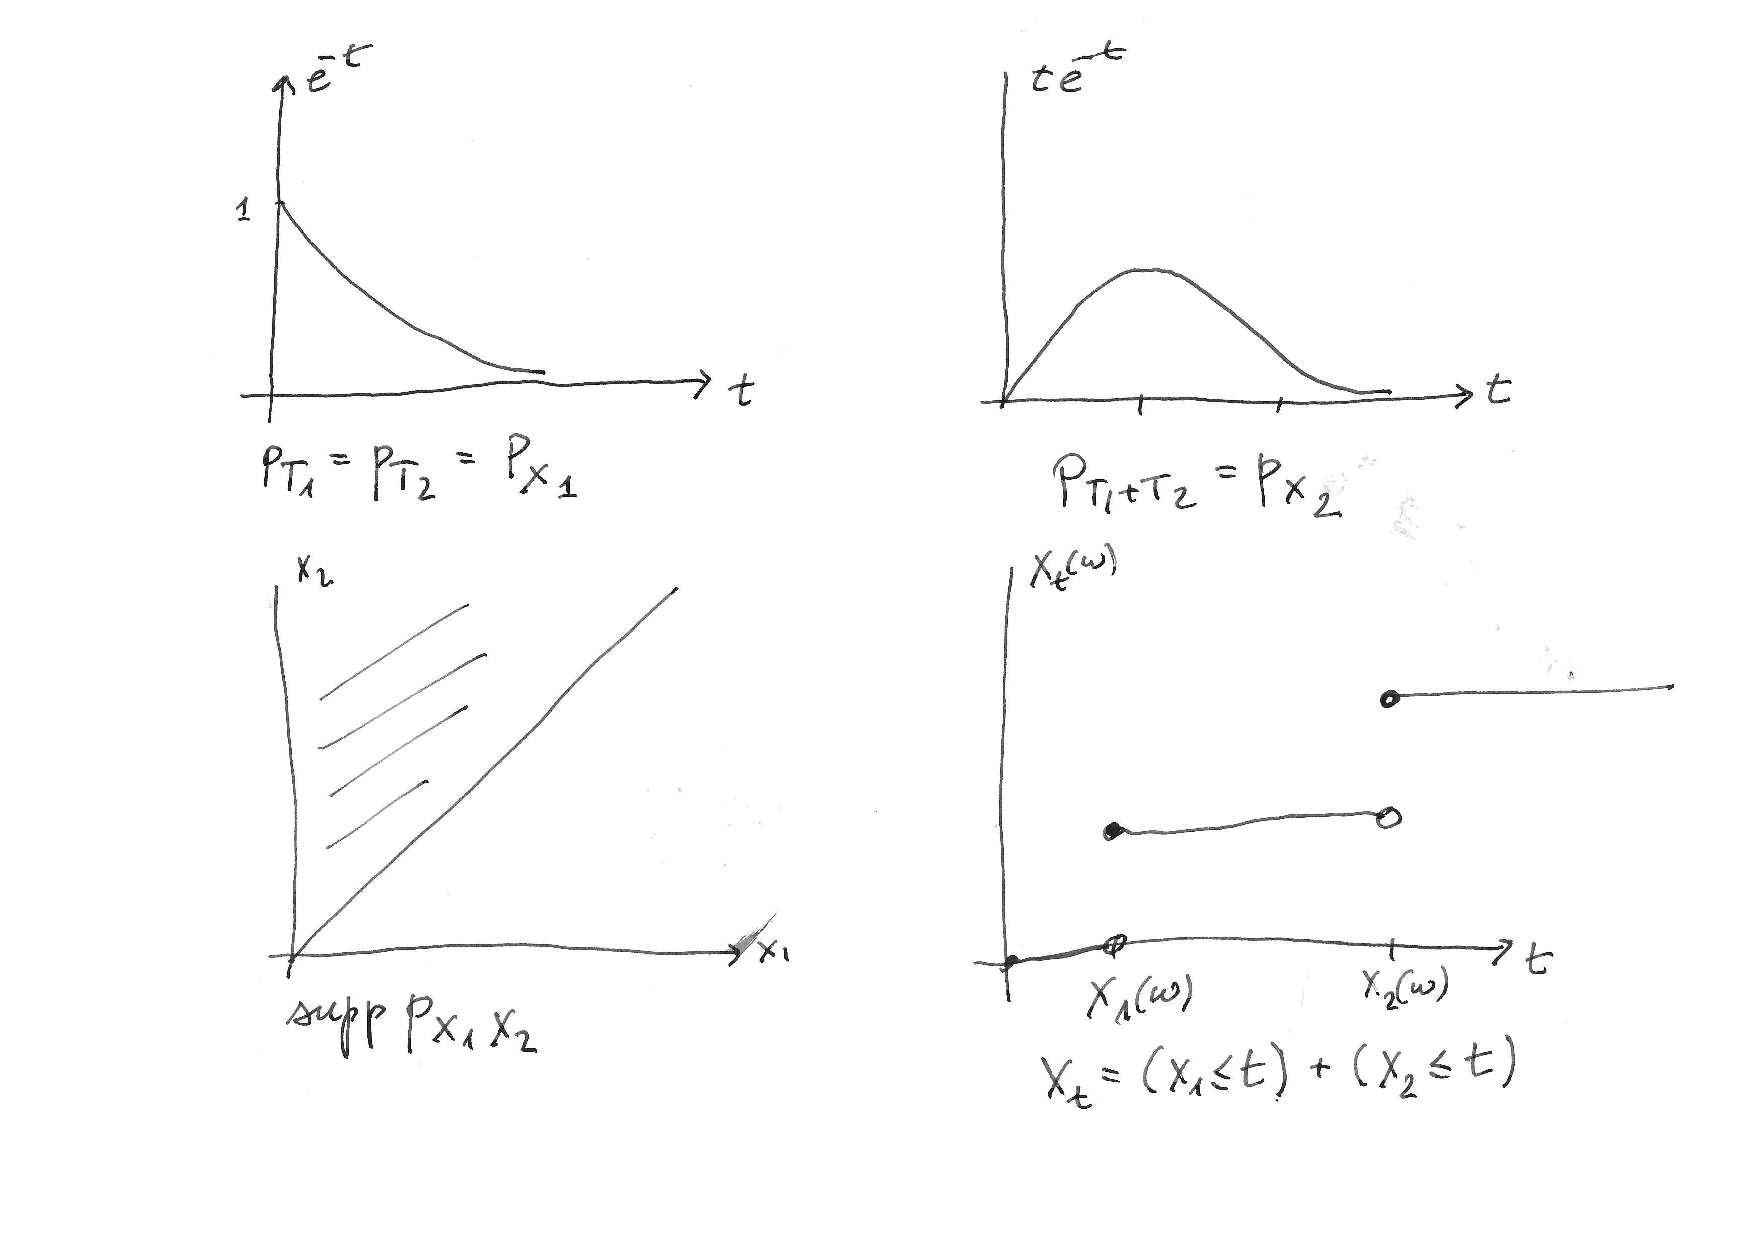
\includegraphics[height=.3\textheight]{pictures/exponential.pdf}
  \caption{Pictures for \cref{ex:exponential}}
\end{figure}
Let $T_1,T_2$
   be independent and Exp$(1)$. That is, the two random variables are
   non-negative, their respective distribution their distribution has
   density $\euler^{-t}$ with respect of the Lebesgue measure on the
   positive real line, and the joint distribution is defined by
   $\expectof {f(T_1,T_2)} = \iint_0^\infty f(t_1,t_2) \
   \euler^{-(t_1+t_2)} dt_1dt_2$. Define $X_1 = T_1$ and
   $X_2=T_1+T_2$. The joint distribution of $(X_1,X_2)$ is
   \begin{multline*}
     \expectof{g(X_1,X_2)} = \expectof {g(T_1,T_1+T_2)} = \\
     \iint_0^\infty g(t_1,t_1+t_2) \euler^{-(t_1+t_2)} \ dt_1dt_2 =
     \iint_{0 \leq x_1 \leq x_2} g(x_1,x_2) \euler^{-x_2} \ dx_1dx_2 = \\
 \iint_0^\infty g(x_1,x_2) \euler^{-x_2}(0 \leq x_1 \leq x_2) \
 dx_1dx_2 \ .  \end{multline*}

It follows that the joint density of $(X_1,X_2)$ is
$$p_{X_1,X_2}(x_1,x_2) = \euler^{-x_2}(0 \leq x_1 \leq x_2) \ .$$ Notice
the support. The marginal densities are, respectively,
\begin{gather*}
  p_{X_1}(x_1) = \int_0^\infty \euler^{-x_2}(0 \leq x_1 \leq x_2)
  \ dx_2 = \int_{x_1}^\infty \euler^{-x_2} \ dx_2 = \euler^{-x_1} (0
  \leq x_1)\ ,\\
  p_{X_2}(x_2) = \int_0^\infty \euler^{-x_2}(0 \leq x_1 \leq x_2) \ dx_1=
  x_2 \euler^{-x_2} (0 \leq x_2) \ .  \end{gather*}

The transition densities are
\begin{gather*}
  p_{X_1|X_2}(x_1|x_2) = \frac{\euler^{-x_2}(0 \leq x_1 \leq x_2)}{x_2
    \euler^{-x_2}(0 \leq x_2)} = x_2^{-1} (0 \leq x_1 \leq x_2) \quad
  \text{if $x_2 \neq 0$} \ , \\ p_{X_2|X_1}(x_2|x_1) =
  \frac{\euler^{-x_2}(0 \leq x_1 \leq x_2)}{\euler^{-x_1}(0 \leq x_1)}
  = \euler^{-(x_2-x_1)}(0 \leq x_1 \leq x_2) \ .
\end{gather*}
The first one is uniform, the second one is a translated exponential.

For each $t \geq 0$ define the random variable
\begin{equation*}
  X_t = (t \geq X_1) + (t \geq X_2) \ .
\end{equation*}
It is a random variable with values $0,1,2$, and the probability
function is
\begin{gather*}
  p_{X_t}(0) = \probof{t < X_1} = \int_t^\infty \euler^{-x_1} \ dx_1 =
  \euler^{-t} \ , \\
  p_{X_t}(1) = \probof{X_1 \leq t < X_2} = \iint_{0 \leq x_1 \leq t < x_2}
  \euler^{-x_2}\ dx_1dx_2 = t\euler^{-t} \ , \\
  p_{X_t}(2) = 1 - \euler^{-t} - t\euler^{-t} \ .
\end{gather*}

Let us compute $\condexp {f(X_2)}{X_t} = \tilde f (X_t)$. The
conditioning variable is finite valued. It follows that
\begin{align*}
  \tilde f(0) &= \frac{\expectof{(X_t=0)f(X_2)}}{\probof{X_t=0}} =
                \frac1{\euler^{-t}} \iint \euler^{-x_2}(t < x_1 \leq
                x_2)\ dx_1dx_2 = \int_t^\infty
                (x_2 - t) \euler^{-(x_2-t)} \ dx_2 \\
  \tilde f(1) &= \frac{\expectof{(X_t=1)f(X_2)}}{\probof{X_t=1}} =
                \frac1{t\euler^{-t}} \iint \euler^{-x_2}(0 \leq x_1 \leq t < x_2)\ dx_1dx_2  \\
  \tilde f(2) &= \frac{\expectof{(X_t=2)f(X_2)}}{\probof{X_t=2}} =
                \frac1{1 - \euler^{-t} - t\euler^{-t}} \iint
                \euler^{-x_2}(0 \leq x_1 \leq x_2 \leq t )\ dx_1dx_2 
\end{align*}
The rest of the computations is left to the reader. This example is an
introduction to Poisson processes, see
\cite[Ch.~5]{ross:2010introduction10}.
\end{example}

\begin{example}[Sum of independent Gaussians]\label{ex:filter}
\begin{figure}
  \centering
  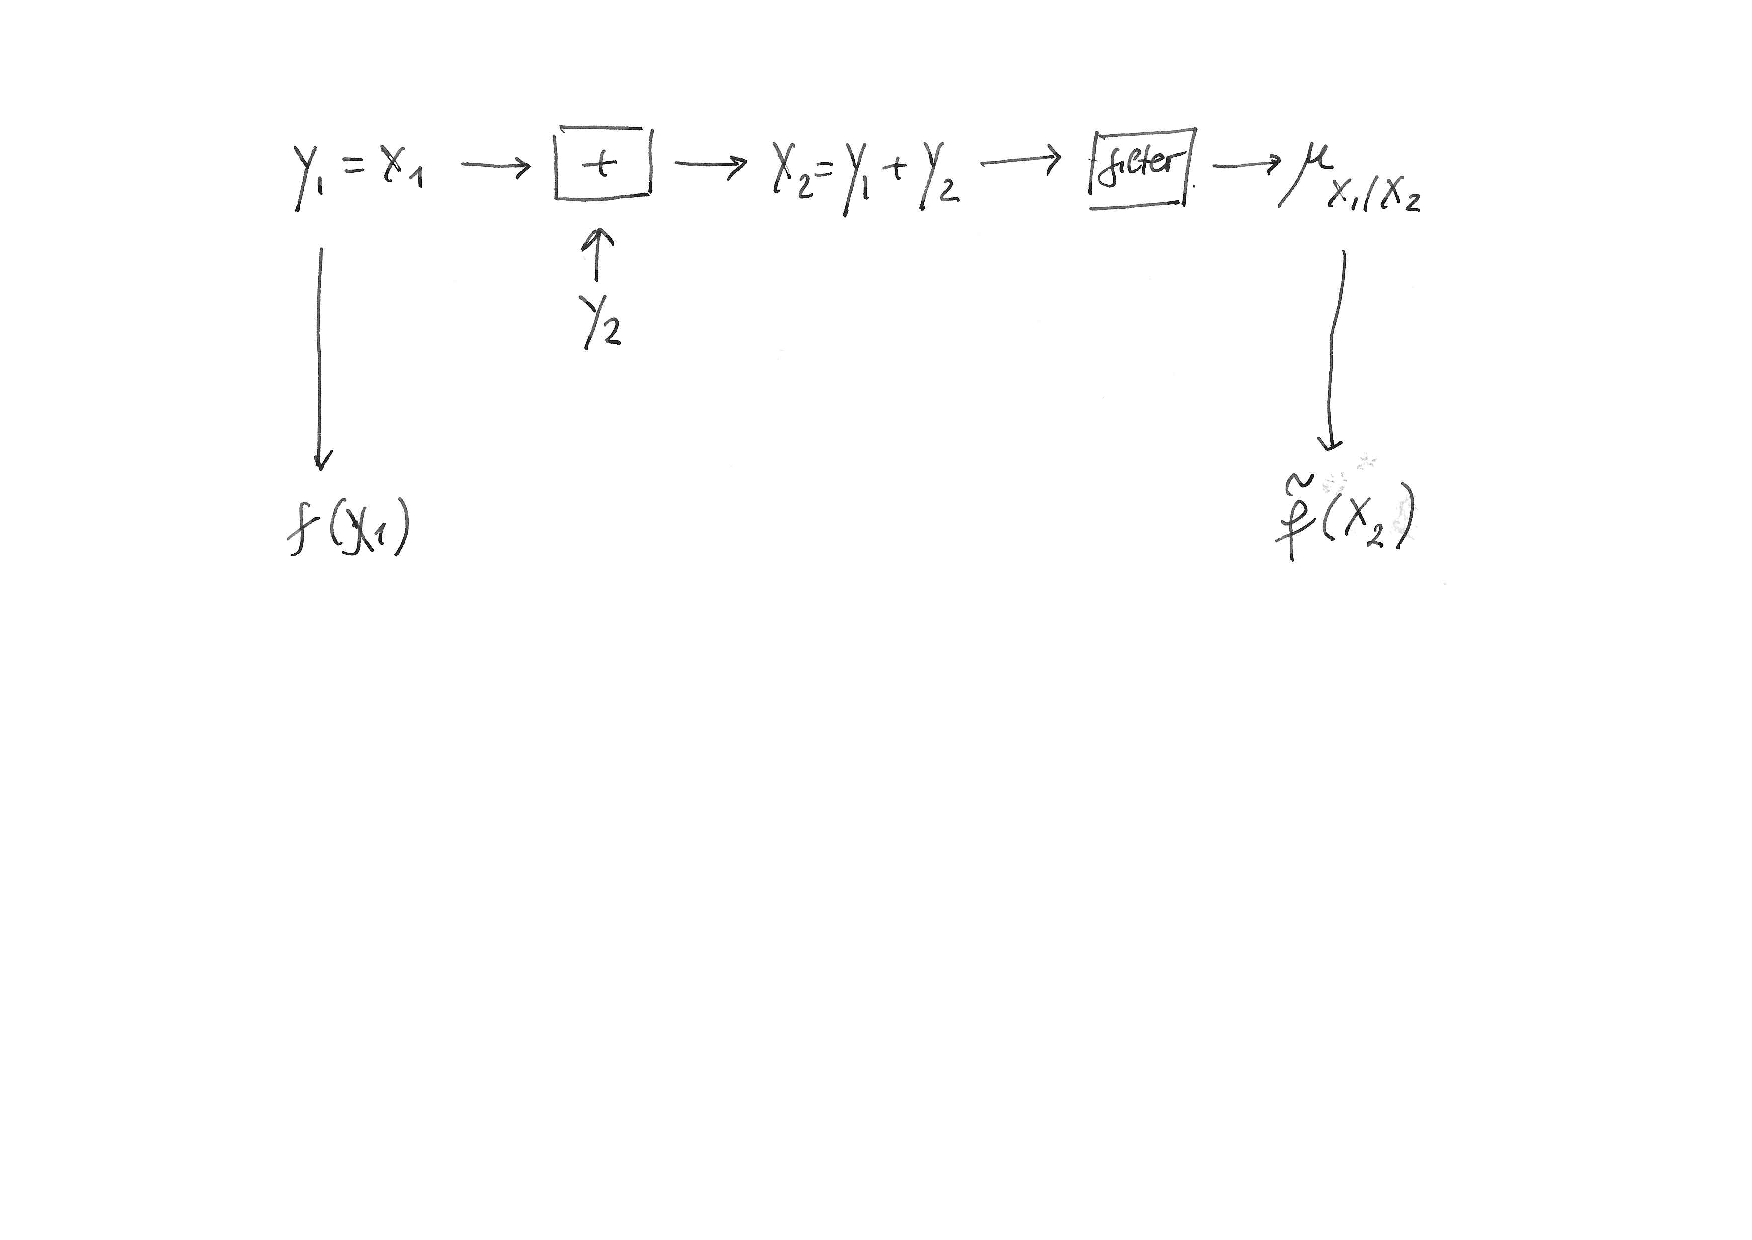
\includegraphics[height=.2\textheight]{pictures/filter.pdf}
  \caption{Additive noise of \cref{ex:filter}\label{fig:filter}}
\end{figure}
If $(Y_1,Y_2)$ are independent standard Gaussians random variables,
find the conditional distribution of $Y_1$ given $Y_1+Y_2$.

Each random variable has distribution
\begin{equation*}
  \expectof{f(Y_i)} = \int f(y) \ \frac1{\sqrt{2\pi}}
  \euler^{-y^2/2}dy \ , \quad i=1,2 \ ,
\end{equation*}
and the joint distribution is
\begin{equation*}
  \expectof {f(Y_1,Y_2)} = \iint f(y_1,y_2) \ \frac1{2\pi} 
  \euler^{-(y_1^2+y_2^2)/2}dy_1dy_2 \ .
\end{equation*}

The distribution of $(X_1,X_2) = (Y_1,Y_1+Y_2)$ is
\begin{multline*}
  \expectof{g(X_1,X_2)} = \expectof{g(Y_1,Y_1+Y_2)} = \\ \iint g(y_1,y_1+y_2) \ \frac1{2\pi} 
  \euler^{-(y_1^2+y_2^2)/2}dy_1dy_2 = 
 \iint g(x_1,x_2) \ \frac1{2\pi} 
  \euler^{-(x_1^2+(x_2-x_1)^2)/2}dx_1dx_2 = \\  \iint g(x_1,x_2) \ \frac1{2\pi}
  \euler^{-(2x_1^2 -2x_1x_2 + x_2^2)/2}dx_1dx_2  \ . 
\end{multline*}

The distribution of $X_2$ is
\begin{multline*}
  \expectof{h(X_2)} = \iint h(x_2) \ \frac1{2\pi} \euler^{-(2x_1^2
    -2x_1x_2 + x_2^2)/2}dx_1dx_2 = \\ \frac1{2\pi}\int dx_2 \ h(x_2)
  \int dx_1 \ \euler^{-(2x_1^2 -2x_1x_2 + x_2^2)/2} = \\ \frac1{2\pi} \int
  dx_2 \ h(x_2) \euler^{-x_2^2/4} \int dx_1 \ \euler^{-(2x_1^2 -2x_1x_2 +
    x_2^2/2)/2} = \\  \frac1{2\pi} \int
  dx_2 \ h(x_2) \euler^{-x_2^2/4} \int dx_1 \ \euler^{-(\sqrt 2 x_1 -
    x_2/\sqrt 2)^2/2} = \\ \frac1{2\pi} \int
  dx_2 \ h(x_2) \euler^{-x_2^2/4} \int dx_1 \ \euler^{-x_1^2} = \int
  h(x_2) \ \frac1{2\sqrt \pi} \euler^{-x_2^2/4} dx_2 \ .  
\end{multline*}

Now it is possible to compute the transition density
\begin{multline*}
  p_{X_1|X_2}(x_1|x_2) = \\ \frac{p_{X_1,X_2}(x_1,x_2)}{p_{X_2}(x_2)} =
  \frac{\frac1{2\pi}
  \euler^{-(2x_1^2 -2x_1x_2 + x_2^2)/2}}{\frac1{2\sqrt \pi}
  \euler^{-x_2^2/4}} = \frac1{\sqrt{\pi}} \euler^{-(2x_1^2 -2x_1x_2 +
    x_2^2/2)/2} = \\ \frac1{\sqrt{\pi}} \euler^{-(x_1-x_2/2)^2} \ .
\end{multline*}

This sort of computations is done in Communication Theory, where $Y_1=X_1$
is the \emph{signal}, $Y_2$ is an additive \emph{noise}, $X_2 =
Y_1+Y_2$ is the \emph{received signal}, $\tilde f (x_2) = \condexp
{f(Y_1)}{x_2}$ is the \emph{filter}, and $f(X_1) - \tilde f(X_2)$ is
the \emph{error}. See \cref{fig:filter}.
\end{example}


\begin{proposition}[Regular version of the conditional expectation]
With the notations above, denoting with $X_1,X_2$ the coordinate
projection, the random variable $\widehat f(X_2) = \int f(x_1,X_2) \
\mu_{1|2}(dx_1|X_2)$ is a version of the conditional expectation
$\condexp {f(X_1,X_2)}{\sigma(X_2)}$.
\end{proposition}

\begin{proof}
  In fact,
  \begin{equation*}
    \expectof {f(X_1,X_2)g(X_2)} = \int \left(\int f(x_1,x_2) \ \mu_{1|2}(dx_1|x_2)\right)g(x_2) \ \mu_2(dx_2) = \expectof {\widehat f(X_2)g(X_2)} \ .
  \end{equation*}
\end{proof}  

\subsection{Markov property and martingales}
\label{sec:markov}

This section contains the introduction to advanced topics in form of
examples. A finite sequence of random variables $X_0, \dots, X_n$ is
called \emph{stochastic process} when the running index $t =
0,1,\dots,n$ is thought of as a running time. The family of
$\sigma$-algebras $\mathcal F_t = \sigma(X_0,\dots,X_t)$ is the
information derived from the cumulative knowledge at time $t$.

We start with the generalization of the assumption $\probof{A \cap C | B} =
\probof{A|B} \probof{C|B}$ and of its equivalent assumption $\probof{C|A
  \cap B} = \probof{C|B}$.

\begin{definition}[Conditional independence in 3 flavours] \ 
  \begin{enumerate}
    \item Let $\mathcal A$,
  $\mathcal B$, $\mathcal C$, be sub-$\sigma$-algebras of the
  probability space $(\Omega,\mathcal F, \mu)$. \emph{$\mathcal A$ and
  $\mathcal C$ are conditionally independent given $\mathcal B$} if
  for all couple $X$ and $Z$ of bounded real random variables measurable
  with respect to $\mathcal A$ and $\mathcal C$, respectively,
  it holds
    \begin{equation*}
      \condexp{XZ}{\mathcal B} = \condexp{X}{\mathcal
        B}\condexp{Z}{\mathcal B} \ .
    \end{equation*}
  \item Let $X$ and $Z$ be random variables of the probability space
    $(\Omega,\mathcal F, \mu)$ and let $\mathcal B$ be
    sub-$\sigma$-algebra. \emph{$X$ and $Z$ are conditionally
      independent given $\mathcal B$} if for all couple $f\circ X$ and
    $h \circ Z$ of bounded real random variables it holds
    \begin{equation*}
      \condexp{f \circ X h \circ Z}{\mathcal B} = \condexp{f \circ
        X}{\mathcal B}\condexp{h \circ Z}{\mathcal B} \ .
    \end{equation*}
  \item Let $X$, $Y$, and $Z$, be random variables of the probability space
    $(\Omega,\mathcal F, \mu)$. \emph{$X$ and $Z$ are conditionally
      independent given $Y$} if for all couple $f\circ X$ and
    $h \circ Z$ of bounded real random variables it holds
    \begin{equation*}
      \condexp{f \circ X h \circ Z}{\sigma(Y)} = \condexp{f \circ
        X}{\sigma(Y)}\condexp{h \circ Z}{\sigma(Y)} \ .
    \end{equation*}
  \end{enumerate}
\end{definition}

\begin{proposition}
  $X$ and $Z$ are conditionally independent given $Y$ if, and only if,
  \begin{equation*}
    \condexp{h(Z)}{\sigma(X,Y)} = \condexp{h(Z)}{\sigma(Y)} \ .
  \end{equation*}
\end{proposition}

\begin{proof}
Write  a version of the conditional expectation in the rhs as
$\widetilde h(Y)$. This random variable $\sigma(X,Y)$-measurable. The
equality means the master equation holds true,
\begin{equation*}
  \expectof{h(Z)\phi(X,Y)} = \expectof{\widetilde h(Y)\phi(X,Y)} \ . 
\end{equation*}
It holds in the particular the case $\phi(x,y) = f(x)g(y)$,
\begin{gather*}
    \expectof{h(Z)f(X)g(Y)} = \expectof{\widetilde h(Y)f(X)g(Y)} \ . 
  \end{gather*}
If we write $\widetilde f(Y) = \condexp{f(X)}{\sigma(Y)}$, the
equality above becomes
\begin{equation*}
     \expectof{h(Z)f(X)g(Y)} = \expectof{\widetilde h(Y)\widetilde f(Y)g(Y)} \ , 
\end{equation*}
which is exactly the conditional independence.

The other implication follows from the backward argument.
  \end{proof}

\begin{example}[Statistical models: sufficiency] Let $(\Omega,\mathcal
  F,\mu)$ be a probability space, $(\Theta,\mathcal T)$ a measurable
  space, and $(x,\theta) \mapsto p(x|\theta)$ be a transition
  density. In Statistics, one talks about a parameter $\theta \in
  \Theta$ and about the statistical model where the expected values are
  computed as
  \begin{equation*}
    \expectat \theta f = \int f(x) \ p(x|\theta)\mu(dx) = \int f(x) \
    \mu_\theta(dx)
  \end{equation*}
for each value of the parameter $\theta$.

Let $T$ be a measurable function of $(\Omega, \mathcal F)$ and
assume that the transition is of the form $p(x|\theta) = \hat
p(T(x)|\theta)$. In this case, the conditional expectation of any real random
variable $Y$ given $T$ does not depend on $\theta$. Precisely, let
$\widetilde Y = \condexpat \mu {Y}{\sigma(T)}$. Then
\begin{equation*}
  \expectat \theta {Yg(T)} = \expectat \mu {Y \hat p(T|\theta) g(T)} =
  \expectat \mu {\widetilde Y p(T|\theta) g(T)} = \expectat \theta
    {\widetilde Y g(T)} \ . 
\end{equation*}
\end{example}

\begin{definition}
A stochastic process $X_0,X_1,\dots,X_n$ is a Markov process if for
each $0 \leq t < n$ and bounded measurable $f$ it holds
\begin{equation*}
       \condexp{f(X_{t+1})}{\sigma(X_0,\dots,X_t)} =
  \condexp{f(X_{t+1})}{\sigma(X_t)} \ .
\end{equation*}
The Markov process has stationary transition $\mu$ if
\begin{equation*}
  \condexp{f(X_{t+1})}{\sigma(X_t)} = \int f(y) \ \mu(dy|X_y) \ .
\end{equation*}

\begin{remark}\label{rem:howto}
In practice, there are two ways to check the Markov condition. First
option is to compute a version $\widetilde f(X_0,\dots,X_t)$ of the lhs and then check if it is
actually a function of $X_t$ only. Second option is compute the
simpler rhs $\widetilde f(X_t)$ and then check it is indeed a version
of the lhs by writing down the relevant master equation.   
\end{remark}

\end{definition}
\begin{definition}[Martingale]
  A stochastic process $(X_0,X_1, \dots, X_n)$ is a martingale if all
  the random variables are integrable and
  \begin{equation*}
    \condexp {X_t}{X_0,\dots,X_{t-1}} = X_{t-1}\ , \quad t=1,\dots,n \ .
  \end{equation*}
Equivalently, 
\begin{equation*}
  \expectof{(X_t-X_{t-1})g_t(X_0,\dots,X_{t-1})} = 0 \ ,
\end{equation*}
for all $t\geq1$ and all bounded measurable $g_t \colon \reals^{t} \to \reals$.
\end{definition}

\begin{example}[Exponential martingale] Let $Z_0,Z_1,\dots$ be a
  sequence of independent random variables such that for each $t$ the
  random variable $\euler^{\sum_{s=0}^tZ_s}$ is integrable. Consider the random
  process $X_t = \expof{\sum_{s=0}^t Z_s - a(t)}$, where $a$ is a
  function on $\set{0,1,\dots}$. For which $a$'s we obtain a
  martingale?

  Notice that $(X_0,\dots,X_t)$ is a function of $(Z_0,\dots,Z_t)$. It
  follows that
  \begin{multline*}
    \expectof{(X_{t} - X_{t-1}) g(X_0,\dots,X_{t-1})} = \\
\expectof{\left(\expof{\sum_{s=0}^t Z_s - a(t)} - \expof{\sum_{s=0}^{t-1}
    Z_s - a(t-1)}\right) \bar g(Z_0,\dots,Z_{t-1})} = \\
\expectof{\left(\expof{Z_t - (a(t)-a(t-1))} - 1\right)\expof{\sum_{s=0}^{t-1}
    Z_s - a(t-1)} \bar g(Z_0,\dots,Z_{t-1})} = \\
\expectof{\left(\expof{Z_t - (a(t)-a(t-1))} - 1\right)} \expectof{\expof{\sum_{s=0}^{t-1}
    Z_s - a(t-1)} \bar g(Z_0,\dots,Z_{t-1})} \ .
  \end{multline*}
This is zero if
\begin{equation*}
  \expectof{\euler^{Z_t} }= \euler^{a(t) - a(t-1)} \ .
\end{equation*}
This is computable as soon as we know the distribution of $Z_t$.
\end{example}

\begin{example}[Stochastic equations]
Given a real integrable random variable $X_0$, functions
\begin{equation*}
  a \colon \set{1,\dots,n} \to \reals \quad \text{and} \quad b \colon
  \reals \times \set{1,\dots,n} \to \reals \ , 
\end{equation*}
and a sequence $Z_1,\dots,Z_n$ of real integrable random
variables such that the sequence $X_0,Z_1,\dots,Z_n$ is independent, define a stochastic process by the recursive equations
\begin{equation*}
  X_t = X_{t-1} + b(X_{t-1},t) + a(t)Z_t \ .
\end{equation*}

Assume moreover that the functions $b(\cdot,t)$ have linear growth,
that is, there exists constants such that
$\aval{b(x,t)} \leq C_0 + C_1\aval x$, $x \in \reals$. We show that
$(X_t)_{t=0}^n$ is an integrable Markov process.

First, let us check the integrability by recursion.
\begin{multline*}
  \expectof{\aval{X_t}} = \expectof{\aval{X_{t-1} + b(X_{t-1},t) +
      a(t)Z_t}} \leq \\ \expectof{\aval{X_{t-1}}} +
    \expectof{\aval{b(X_{t-1},t)}} + \expectof{\aval{a(t)Z_t}} \leq
  \\ \expectof{\aval{X_{t-1}}} +
    C_0 + C_1 \expectof{\aval{X_{t-1}}} + \aval{a(t)}
    \expectof{\aval{Z_t}} <  \infty
  \end{multline*}

Second, let us observe that each $X_{t}$ is a function of
$X_0,Z_1,\dots,Z_{t}$, so that $(X_0,\dots,X_{t-1}$ and $Z_t$ are independent.
That is, the joint distribution of $(X_0,\dots,X_{t-1},Z_t)$ factors as
\begin{equation*}
  \mu_{(X_0,\dots,X_{t-1},Z_t)} = \mu_{(X_0,\dots,X_{t-1})} \otimes
  \mu_{Z_t} \ ,
\end{equation*}
and
\begin{equation*}
  \expectof{f(X_0,\dots,X_{t-1},Z_t)} = \expectof{\int
    f(X_0,\dots,X_{t-1},z) \ \mu_{Z_t}(dz)}
\end{equation*}
for all $f$ because of Fubini's theorem.

In conclusion, let us check the Markov property. For each
bounded $\phi \colon \reals$ and bounded $g \colon \reals^t$ it holds,
\begin{multline*}
  \expectof{(\phi(X_t)g(X_0,\dots,X_{t-1})} = \\
  \expectof{\phi(X_{t-1} + b(X_{t-1},t) +
    a(t)Z_t)g(X_0,\dots,X_{t-1})} = \\
  \expectof{\left(\int \phi(X_{t-1} + b(X_{t-1},t) +
    a(t)z) \ \mu_{Z_t}(dz)\right) g(X_0,\dots,X_{t-1})}  \ .
\end{multline*}
We have found that
\begin{equation*}
  \condexp {\phi(X_t)}{X_0,\dots,X_{t-1}} = \int \phi(X_{t-1} + b(X_{t-1},t) +
    a(t)z) \ \mu_{Z_t}(dz) \ ,
\end{equation*}
which is indeed a function of $X_{t-1}$ only with
\begin{equation*}
  \widetilde \phi(x_{t_1}) = \int \phi(x_{t-1} + b(x_{t-1},t) +
    a(t)z) \ \mu_{Z_t}(dz) = \expectof{\phi(x_{t-1} + b(x_{t-1},t) +
    a(t)Z_t} \ .
\end{equation*}
To find explicitly the transition, one must compute for each $x_t$ the
distribution of  the random variable $x_{t-1} + b(x_{t-1},t) +
    a(t)Z_t$.
\end{example}

\begin{example}
  [Compensator] Let $X_0,X_1,\dots,X_n$ be a real integrable random
  process and define $\mathcal F_t = \sigma(X_0,\dots,X_t)$. A process
  $A_0,\dots,A_n$ is predictable wrt $(\mathcal F_t)_{t=0}^n$ if
  $A_0=0$ and $A_t$
  is $F_{t-1}$-measurable, $t \geq 1$. It is a predictable compensator of
  $X_0,X_1,\dots,X_n$ if $(X_t - A_t)_{t=0}^n$ is a martingale.

  Write $M_t = X_t - A_t$ and observe that $(M_0,\dots,M_t)$ is
  $\mathcal F_t$-measurable. It follows that
  \begin{equation*}
0 =\condexp {M_t-M_{t-1}}{\mathcal F_{t-1}} = \condexp
{X_t-X_{t-1}}{\mathcal F_{t-1}} - (A_t - A_{t-1}) \ ,
  \end{equation*}
which, in turn, implies
\begin{equation*}
  A_t = \sum_{s=1}^t (A_s - A_{s-1}) = \sum_{s=1}^t \condexp
{X_t-X_{t-1}}{\mathcal F_{t-1}} \ .  
\end{equation*}

\end{example}
\begin{example}[Martingale problem]
Let $(X_t)_{t=0}^n$ be a Markov process with stationary transition
$\mu$. Let us compute the predictable compensator of
$(\phi(X_t))_{t=0}^n$, $\phi$ bounded.

We have
\begin{multline*}
  \expectof {(\phi(X_t) -
    \phi(X_{t-1}))g(\phi(X_0),\dots,\phi(X_{t-1}))} = \\ \expectof
  {(\int \phi(y) \ \mu(dy|X_{t-1}) -
    \phi(X_{t-1}))g(\phi(X_0),\dots,\phi(X_{t-1}))} \ , 
\end{multline*}
so that the predictable compensator is
\begin{equation*}
 A^\phi_t = \sum_{s=1}^t \int (\phi(y) - \phi(X_{t-1}))\
 \mu(dy|X_{t-1}) \ .
\end{equation*}

\emph{Conversely}, given a random process $(X_t)_{t=0}^n$ and a
transition $\mu$, if for all bounded $\phi$ the process defined by
\begin{equation*}
  M^\phi_t = \phi(X_t) - A^\phi_t 
\end{equation*}
is a martingale, then $(X_t)_{t=0}^n$ is a Markov process with
stationary transition $\mu$.

In fact,
\begin{multline*}
  \condexp{\phi(X_t)}{X_0,\dots,X_{t-1}} =  \condexp{M^\phi_t +
    A^\phi_t}{X_0,\dots,X_{t-1}} = \\
  \condexp{M^\phi_t}{X_0,\dots,X_{t-1}}  +
    A^\phi_t = M^\phi_{t-1} + A^\phi_t = \phi(X_{t-1}) - A^\phi_{t-1}
    + A^{\phi}_{t} = \\ \int \phi(y) \ \mu(dy|X_{t-1}) \ .
\end{multline*}
This way to define the Markov property is called \emph{Martingale problem}.
\end{example}

\bibliography{tutto}%
\bibliographystyle{amsplain}

\end{document}

